%% ============================================================
%% Lambda-EG: A Screened Scalar-Tensor Framework for
%% Low-Acceleration Gravitational Phenomenology
%% J. P. Figueroa Torres
%% Lambda-EG framework paper
%% ============================================================

\documentclass[11pt,a4paper]{article}

\usepackage[T1]{fontenc}
\usepackage[utf8]{inputenc}

\usepackage{geometry}
\geometry{margin=2.5cm}

\usepackage{amsmath,amssymb,amsfonts,mathtools}
\usepackage{bm}
\usepackage{graphicx}
\graphicspath{{figuras/}{./}}
\usepackage{booktabs}
\usepackage{xcolor}
\usepackage{hyperref}
\usepackage{cite}
\usepackage{enumitem}

\usepackage{amsthm}
\newtheorem{theorem}{Theorem}[section]
\newtheorem{remark}{Remark}[section]

% For Dirac slash notation
\usepackage{cancel}
\newcommand{\slashed}[1]{\cancel{#1}}

\hypersetup{
  colorlinks = true,
  linkcolor  = blue,
  citecolor  = blue,
  urlcolor   = blue
}

%% ============================================================
\title{\textbf{$\Lambda$-EG: A Screened Scalar--Tensor Framework\\
for Low-Acceleration Gravitational Phenomenology}}

\author{J.~P.~Figueroa Torres\\[4pt]
\small Independent Researcher\\
\small Guadalajara, Jalisco, Mexico}

\date{April 2026}
%% ============================================================

\begin{document}

\maketitle

\begin{abstract}
We present $\Lambda$-EG (Lambda Emergent Gravity), a covariant scalar--tensor
framework in which a k-essence field $\phi$ recovers General Relativity in screened
high-acceleration environments while reproducing modified dynamics in the
low-acceleration regime relevant to galactic phenomenology.
The critical acceleration scale
\begin{equation*}
  g_{\rm crit} = \frac{cH_0}{4\pi^2\sqrt{3}} \approx 9.58\times10^{-12}\ \text{m\,s}^{-2}
\end{equation*}
is motivated, without free parameters, primarily by the spectral geometry of the
De~Sitter horizon: the first non-zero Beltrami--Laplace eigenvalue on $S^3$
($\lambda_1 = 3$) fixes the $\sqrt{3}$, while the $4\pi^2$ factor follows from the
horizon heat-kernel measure. The Dirac--Lichnerowicz curvature term $R/4$ on $S^4$
yields the same value under a common curvature-radius normalization, as a related
geometric consistency check. A complete variational principle unifying these
ingredients remains an open aspect of the framework.

Starting from a k-essence action $\mathcal{L}_\phi = -a_*^2 F(X)$ with
$X = (\partial\phi)^2/a_*^2$, we derive three mutually consistent field equations:
(i)~the covariant k-essence equation; (ii)~the modified Einstein equations with
k-essence source; (iii)~the non-relativistic limit of a screened scalar--tensor
structure, in which the deep-MOND relation $V^4 = GM_{\rm bar}\,a_0$
(with $a_0 = 4\pi\,g_{\rm crit}$) emerges asymptotically when the scalar
contribution dominates, while the Newtonian regime is recovered through screening.
The pure kinetic branch $F(X)\propto X^{3/2}$ corresponds to the deep-MOND (infrared)
limit; the complete kinetic function, used consistently throughout, interpolates to
Newtonian dynamics at high acceleration and yields $\mu(x)=x/\sqrt{1+x^2}$.
In dense environments a density-dependent screening potential traps the field near a
local minimum, suppressing the scalar force through a thin-shell mechanism that
satisfies Cassini PPN bounds ($|\gamma - 1| \lesssim 2.3\times10^{-5}$) for
sufficiently large coupling ($\alpha \gtrsim 8\times10^{6}$, with
$F_\phi/F_N \propto \alpha^{-5/3}$).
For the asymptotic kinetic branch $F(X)\propto X^{3/2}$, scalar perturbations
propagate at constant subluminal speed $c_s^2 = 1/2$, ensuring strict hyperbolicity.
A topological transition radius $r_t = \sqrt{GM/g_{\rm crit}}$ separates the
screened and unscreened dynamical domains.

Observational validation against 184 galaxies from the SPARC and LITTLE~THINGS
catalogs is reported in the companion papers~\cite{PaperI,PaperII}. The present
paper provides the complete field-theoretic foundation. Open problems are stated
explicitly.
\end{abstract}

\tableofcontents
\newpage

%%====================================================
\section{Introduction}
\label{sec:intro}

General Relativity (GR) is confirmed to high precision from Solar-System to compact-object
scales. At galactic and larger scales, the standard $\Lambda$CDM paradigm invokes
non-baryonic dark matter to account for observed mass discrepancies. Despite its
considerable empirical success, the microphysical identity of dark matter remains
unknown.

Several observational regularities motivate continued investigation of the gravitational
sector. The radial acceleration relation \cite{McGaugh2016}, the baryonic
Tully--Fisher relation (BTFR)~\cite{McGaugh2000}, and the flatness of rotation curves
in low-surface-brightness (LSB) galaxies~\cite{Rubin1980} all suggest that galactic
dynamics contains structure beyond purely Newtonian expectations when baryonic mass
alone is considered. The small intrinsic scatter ($\sigma\approx0.07$~dex) of the BTFR
is particularly constraining: it implies a tight coupling between baryonic mass and
asymptotic orbital velocity that is difficult to accommodate naturally within stochastic
dark-matter halo formation \cite{McGaugh2000}.

Modified-gravity proposals including MOND~\cite{Milgrom1983}, AQUAL~\cite{Bekenstein1984},
TeVeS, screened scalar-tensor theories~\cite{Khoury2004, Babichev2009}, and emergent
gravity scenarios~\cite{Verlinde2017} have addressed different aspects of this problem.
The present paper introduces $\Lambda$-EG (Lambda Emergent Gravity), a compact covariant
framework combining three properties:
\begin{enumerate}[label=(\roman*)]
\item recovery of GR in screened high-acceleration environments;
\item modified dynamics in the low-acceleration regime, reproducing flat rotation
      curves and BTFR scaling;
\item a critical acceleration scale $g_{\rm crit}$ derived from the spectral geometry
      of the De~Sitter horizon, linking infrared gravitational phenomenology to the
      cosmological background without free parameters.
\end{enumerate}

Figure~\ref{fig:concept} summarizes the logical structure of the framework, from the
action to the observational phenomenology. The fundamental dynamical object of
$\Lambda$-EG is the scalar field $\phi$: the spectral construction of
Section~\ref{sec:gcrit} fixes the critical scale, while decoherence in the
De~Sitter background provides its physical interpretation. What distinguishes $\Lambda$-EG
from a scalar--tensor theory with a phenomenologically chosen potential is precisely this:
the low-acceleration scale $g_{\rm crit}$ is \emph{not} a free parameter tuned to galaxies,
but is fixed by the spectral geometry of the cosmological horizon together with the present
Hubble rate $H_0$. The empirical MOND scale thereby acquires a geometric origin,
$a_0 = 4\pi\,g_{\rm crit}$.

This geometric origin yields a prediction that distinguishes $\Lambda$-EG from MOND. In MOND
the acceleration scale $a_0$ is a universal constant; in $\Lambda$-EG it inherits the
cosmological background, $g_{\rm crit}(z)\propto H(z)$, so the zero-point of the BTFR evolves
with redshift as $V\propto[H(z)/H_0]^{1/4}$. This evolution is \emph{absent} in standard MOND
and is testable with high-redshift kinematics (e.g.\ JWST/JADES); a second, independent
discriminator is the acceleration scale probed by wide binary stars, which separates
$g_{\rm crit}$ from $a_0$ (Gaia). These provide concrete tests where $\Lambda$-EG and MOND
diverge, rather than merely reproducing shared low-redshift phenomenology. We
flag at the outset that $g_{\rm crit}(z)\propto H(z)$ is the
\emph{instantaneous--de Sitter} reading of the spectral derivation of
Section~\ref{sec:gcrit}: there $g_{\rm crit}$ is set by the curvature of the
horizon, and the identity $R=12H^2$ that turns curvature into Hubble rate is
exact in de Sitter space only. The covariant alternative is discussed where
the evolution is derived; it is the reading favoured by the data, but it is a
reading and not a consequence.

The field-theoretic structure and geometric derivation of $g_{\rm crit}$ are the primary
content of this paper. Observational validation against galaxy rotation curves and
predictions for the cosmological evolution of the BTFR are presented in the companion
papers~\cite{PaperI,PaperII}, to which we refer for all numerical confrontation with data.

We adopt units $c = 1$ where convenient and restore factors of $c$ in final expressions.
The signature is $(-,+,+,+)$. We use $H_0 = 67.4\ \text{km\,s}^{-1}\text{Mpc}^{-1}$
(Planck~2020~\cite{Planck2020}) throughout.

%%====================================================
\section{The \texorpdfstring{$\Lambda$}{Lambda}-EG Action and Field Equations}
\label{sec:action}

\subsection{Action}
\label{subsec:action}

We consider a real scalar field $\phi$ minimally coupled to gravity, with a
density-dependent screening potential $V(\phi,\rho)$:
\begin{equation}
  S = \int d^4x\sqrt{-g}\left[\frac{R}{16\pi G} - \frac{\Lambda}{8\pi G}
  - a_*^2 F(X) - V(\phi,\rho)\right] + S_{\rm mat},
  \label{eq:action}
\end{equation}
where
\begin{equation}
  X = \frac{(\partial\phi)^2}{a_*^2} = \frac{g^{\mu\nu}\partial_\mu\phi\,\partial_\nu\phi}{a_*^2}
\end{equation}
is the dimensionless kinetic invariant, and $a_* \equiv g_{\rm crit}$ is the critical
acceleration scale fixed by De~Sitter spectral geometry (Section~\ref{sec:gcrit}).
The normalization by $a_*^2$ is not optional: without it the vacuum energy density
develops as $\rho_\phi\sim H_0^3/G$ instead of the physical $\rho_\Lambda\sim H_0^2/G$,
yielding an inconsistent cosmological limit.

The action~(\ref{eq:action}) belongs to the k-essence class~\cite{ArmendarizPicon1999},
with $a_*$ fixed by spectral geometry rather than fitted to data. The screening potential
$V(\phi,\rho)$ is specified in Section~\ref{sec:screening}.

\subsection{Field equations}
\label{subsec:fieldeqs}

Variation of~(\ref{eq:action}) with respect to $g^{\mu\nu}$ gives the modified Einstein
equations:
\begin{equation}
  G_{\mu\nu} + \Lambda g_{\mu\nu}
  = 8\pi G\left(T_{\mu\nu}^{(\rm mat)} + T_{\mu\nu}^{(\phi)}\right),
  \label{eq:einstein}
\end{equation}
with scalar stress-energy tensor
\begin{equation}
  T_{\mu\nu}^{(\phi)}
  = 2F'(X)\,\partial_\mu\phi\,\partial_\nu\phi
  - g_{\mu\nu}\,a_*^2 F(X)
  - g_{\mu\nu} V,
  \label{eq:Tphi}
\end{equation}
where $F'(X)\equiv dF/dX$. Variation with respect to $\phi$ yields the covariant
k-essence equation:
\begin{equation}
  \nabla_\mu\!\left[F'(X)\,\partial^\mu\phi\right] = \frac{\partial V}{\partial\phi}.
  \label{eq:kessence}
\end{equation}

In the non-relativistic quasi-static limit (Section~\ref{subsec:NR_limit}), with
$x \equiv |\nabla\Phi|/a_*$ and $\Phi$ the Newtonian potential, the three field
equations reduce to a mutually consistent set:
\begin{align}
  \text{(k-essence NR):}\quad &\nabla\cdot\!\left[F'(x^2)\,\nabla\Phi\right] = 4\pi G\rho,
  \label{eq:NR_kessence}\\[4pt]
  \text{(modified Poisson):}\quad &\nabla\cdot\!\left[\mu(|\nabla\Phi|/a_*)\,\nabla\Phi\right]
  = 4\pi G\rho,\quad \mu(x) = F'(x^2),
  \label{eq:AQUAL}\\[4pt]
  \text{(BTFR limit):}\quad &V^4 = G M_{\rm bar}\,a_0,\quad a_0 = 4\pi\,g_{\rm crit},
  \label{eq:BTFR}
\end{align}
where equation~(\ref{eq:AQUAL}) is the AQUAL equation of Bekenstein and Milgrom~\cite{Bekenstein1984}
and equation~(\ref{eq:BTFR}) holds in the deep collective regime $x\ll 1$.

\subsection{Fixing the kinetic function}
\label{subsec:FX}

The MOND interpolating condition $\mu(x)\sim x$ for $x\ll 1$ fixes the deep-MOND
(infrared) branch of the kinetic function,
\begin{equation}
  F'(X)\sim X^{1/2} \implies F_{\rm IR}(X) = \tfrac{2}{3}\,X^{3/2},
  \qquad \mu(x)=F_{\rm IR}'(x^2)=x,
  \label{eq:F_AQUAL}
\end{equation}
which reproduces asymptotically flat rotation curves at low acceleration. This pure cubic
form captures \emph{only} the deep-MOND limit and gives $\mu(x)=x$; it does not by itself
recover Newtonian dynamics. The complete kinetic function used throughout,
\begin{equation}
  F(X) = \sqrt{X(1+X)} - \operatorname{arcsinh}\!\sqrt{X},
  \qquad \mu(x)=F'(x^2)=\frac{x}{\sqrt{1+x^2}},
  \label{eq:F_full}
\end{equation}
interpolates smoothly between this limit and Newtonian dynamics, with $F(X)\to X$ and
$\mu\to 1$ at $x\gg 1$ (Figure~\ref{fig:Fphi}). The dynamical selection of this branch is
discussed in the following subsection.

\subsection{Dynamical selection of the kinetic branch}
\label{subsec:FX_attractor}

The functional form $F(X) \propto X^{3/2}$ identified in
equation~(\ref{eq:F_AQUAL}) is not an arbitrary choice imposed to reproduce
MOND phenomenology. It emerges as the stable branch dynamically selected by the
evolution of the scalar field in the low-acceleration regime.

To see this, consider the vacuum ($\rho \to 0$), quasi-static, spherically
symmetric limit of the k-essence equation~(\ref{eq:kessence}):
\begin{equation}
  \frac{1}{r^2}\frac{d}{dr}\left(r^2 F_X \phi'\right) = 0,
\end{equation}
which integrates to
\begin{equation}
  F_X \phi' = \frac{C}{r^2},
\end{equation}
where $F_X \equiv dF/dX$ and $C$ is an integration constant fixed by the
baryonic mass distribution. Defining $X = (\phi')^2$, this relation becomes
\begin{equation}
  F_X \sqrt{X} \propto \frac{1}{r^2}.
\end{equation}
For a general power-law kinetic function $F(X)\sim X^n$, one has
$F_X \sim X^{n-1}$, leading to
\begin{equation}
  X^{n - 1/2} \propto \frac{1}{r^2}.
\end{equation}
Solving for the radial dependence,
\begin{equation}
  X(r) \propto r^{-\frac{2}{n - 1/2}},
  \qquad
  \phi'(r) \propto r^{-\frac{1}{n - 1/2}}.
\end{equation}
Asymptotically flat rotation curves require $\phi'(r) \propto r^{-1}$,
which uniquely fixes
\begin{equation}
  n = \frac{3}{2}.
\end{equation}
This establishes that $F(X)\propto X^{3/2}$ is the only kinetic branch
compatible with stationary solutions exhibiting flat circular velocities.

To address whether this branch is dynamically selected, consider the
non-equilibrium scalar-field dynamics derived in Paper~II~\cite{PaperII},
which introduces a dissipative term associated with cosmological expansion.
In the comoving frame, perturbations $\delta X$ around a background solution
satisfy a schematic evolution equation of the form
\begin{equation}
  \delta X'' + \Gamma\,\delta X' + \mathcal{M}^2(X)\,\delta X = 0,
\end{equation}
where $\Gamma \sim 3H_0 > 0$ represents Hubble friction and $\mathcal{M}^2$
is an effective stability operator determined by $F(X)$.
The presence of positive friction implies that unstable or non-stationary
branches decay toward dynamically stable configurations. Evaluating the
effective restoring term $\mathcal{M}^2$ for perturbations around power-law
solutions shows that only the branch $n = 3/2$ yields a non-negative operator,
ensuring that $\delta X \to 0$ at large radii. Deviations from this branch
either decay toward it or fail to produce stationary solutions compatible
with finite-energy boundary conditions.

Therefore, the asymptotic form
\begin{equation}
  F(X) = \frac{2}{3}X^{3/2}
\end{equation}
is dynamically selected as an attractor of the scalar-field evolution in
the infrared regime. The combined requirements of (i)~regularity,
(ii)~finite energy, (iii)~flat rotation curves, and (iv)~dissipative relaxation
uniquely select the $X^{3/2}$ branch, removing the apparent degeneracy in the
choice of the kinetic function.

\begin{remark}
A complete analytic derivation of the stability operator $\mathcal{M}^2(X)$
confirming that $n=3/2$ is the unique non-negative branch is deferred to
future work.  The selection is confirmed observationally by the dual falsification
test of Paper~I \cite{PaperI}, which rules out $n\neq 3/2$ at median velocity
error $<20\%$ across the collective galaxy subsample.
\end{remark}

\subsection{Non-relativistic limit and screened scalar--tensor structure}
\label{subsec:NR_limit}

We now derive the non-relativistic (NR) limit of the covariant field equations
explicitly, showing how the deep-MOND (AQUAL) behaviour emerges asymptotically within a
screened scalar--tensor structure.

We consider weak-field, quasi-static configurations around Minkowski space,
\begin{equation}
  g_{\mu\nu} = \eta_{\mu\nu} + h_{\mu\nu}, \qquad |h_{\mu\nu}| \ll 1,
\end{equation}
with the standard identification of the Newtonian potential,
\begin{equation}
  h_{00} = -2\Phi_N, \qquad h_{ij} = 2\Phi_N \delta_{ij}.
\end{equation}
In this regime, time derivatives are subdominant compared to spatial gradients,
$\partial_t \phi \ll \nabla \phi$, and the kinetic scalar reduces to
\begin{equation}
  X = \frac{(\nabla \phi)^2}{a_*^2}.
\end{equation}
The covariant k-essence equation~(\ref{eq:kessence}) then reduces to
\begin{equation}
  \nabla \cdot \left( F_X \nabla \phi \right) = \frac{\partial V_{\rm eff}}{\partial \phi}.
\end{equation}
In the low-density regime outside screened regions, the effective potential
gradient is negligible,
\begin{equation}
  \frac{\partial V_{\rm eff}}{\partial \phi} \approx 0,
\end{equation}
leading to
\begin{equation}
  \nabla \cdot \left( F_X \nabla \phi \right) = 0.
\end{equation}
The physical gravitational potential is defined as the sum of the Newtonian
contribution and the scalar-field correction,
\begin{equation}
  \Phi = \Phi_N + c^2 \alpha \phi,
\end{equation}
so that test-particle acceleration is governed by $\mathbf{g} = -\nabla \Phi$.
Using the baryonic Poisson equation,
$\nabla^2 \Phi_N = 4\pi G \rho$,
and combining both contributions, we obtain
\begin{equation}
  \nabla \cdot \left[ \nabla \Phi_N + c^2 \alpha F_X \nabla \phi \right]
  = 4\pi G \rho.
\end{equation}
The full non-relativistic equation obtained above is \emph{not} identical to the AQUAL
equation: it retains separate Newtonian and scalar contributions. In the low-acceleration
(deep-MOND) regime, however, the scalar contribution dominates,
$|\nabla\Phi|\to|\nabla(c^2\alpha\phi)|$, and defining the interpolating function
\begin{equation}
  \mu\!\left(\frac{|\nabla \Phi|}{a_*}\right) \equiv F_X,
\end{equation}
the equation reduces asymptotically to the AQUAL form
\begin{equation}
  \nabla \cdot \left[
    \mu\!\left(\frac{|\nabla \Phi|}{a_*}\right)\nabla \Phi
  \right]
  = 4\pi G \rho,
\end{equation}
of Bekenstein and Milgrom~\cite{Bekenstein1984}. The standard AQUAL behaviour thus emerges
as the deep-MOND asymptotic limit of a screened scalar--tensor structure, not as an exact
identity of the full non-relativistic equations; the Newtonian regime is recovered through
the screening mechanism, which suppresses the scalar contribution at high acceleration. In
this sense the MOND-like modification arises dynamically from the covariant theory rather
than being imposed phenomenologically.

%%====================================================
\section{Origin of the Critical Scale: Spectral Geometry of De~Sitter}
\label{sec:gcrit}

The value of $a_*$ is not a free parameter. The relevant geometry is not chosen among
manifolds: $S^3$ is the spatial section of De~Sitter space, the maximally symmetric
late-time attractor of an accelerating universe, so the construction is fixed by the
physical vacuum rather than by convenience. We obtain the scale \emph{primarily} from the
scalar spectral gap on this $S^3$ (Section~\ref{subsec:BL}), with an \emph{independent}
geometric consistency check from the curvature term on $S^4$ (Section~\ref{subsec:DL});
both give
\begin{equation}
  \boxed{g_{\rm crit} = \frac{cH_0}{4\pi^2\sqrt{3}}\approx 9.58\times10^{-12}\ \text{m\,s}^{-2}}
  \label{eq:gcrit}
\end{equation}
with $H_0 = 67.4\ \text{km\,s}^{-1}\text{Mpc}^{-1}$ \cite{Planck2020}. The relevant infrared
scale is the \emph{present} Hubble rate because the coherence length set by the De~Sitter
thermal bath equals the current horizon radius, $\ell_{\rm dec}\simeq c/H_0$; consequently
$g_{\rm crit}(z)\propto H(z)$, the origin of the redshift dependence tested at high $z$.
Why $H_0$ takes its observed value is the cosmological-constant problem and is not
addressed here.

\subsection{Primary derivation: scalar spectral gap on \texorpdfstring{$S^3$}{S3}}
\label{subsec:BL}

The De~Sitter horizon has spatial section $S^3$ with Hubble radius $R_H = c/H_0$.
The Beltrami--Laplace operator $\Delta_{S^3}$ has eigenvalues
\begin{equation}
  \lambda_\ell^{S^3} = \ell(\ell+2), \quad \ell = 0,1,2,\ldots
\end{equation}
The $\ell = 0$ mode is the constant function: it carries zero energy and provides no
dynamical scale. The first non-trivial mode is $\ell = 1$ by topology, with
\begin{equation}
  \lambda_1^{S^3} = 3 \implies \sqrt{\lambda_1^{S^3}} = \sqrt{3}.
\end{equation}
The factor $4\pi^2 = 2\,\text{Vol}(S^3)$ arises from the horizon heat-kernel measure
($\text{Vol}(S^3) = 2\pi^2$), reflecting the four-dimensionality of De~Sitter spacetime.
Combining the spectral gap $\sqrt{\lambda_1^{S^3}} = \sqrt{3}$ with this measure fixes
the scale,
\begin{equation}
  g_{\rm crit} = \frac{cH_0}{4\pi^2\sqrt{3}}.
\end{equation}
This spectral/heat-kernel construction is presented as the primary route \emph{motivating}
the numerical factor; a complete variational principle unifying the spectral gap and the
measure into a single derivation remains an open aspect of the framework.
Three independent arguments establish the inevitability of $\ell = 1$: (a)~topological
(it is the first mode with nonzero eigenvalue); (b)~Bunch-Davies projection from $S^4$
onto $S^3$ (the $\ell_4=0$ mode does not project onto $\ell_3=1$, while $\ell_4=1$
does, verified numerically); (c)~geodesic embedding ($S^3\subset S^4$ is totally
geodesic, so the induced operator carries eigenvalues $\lambda_\ell^{S^3}$ without
extrinsic correction).
The resulting number is therefore rigid: a different manifold or a different mode would
change it (the first non-zero Laplace eigenvalues on $S^2$ and $S^4$ are $2$ and $4$, not
$3$), so $\sqrt{3}$ is specific to the $\ell=1$ mode on the $S^3$ section of De~Sitter and
is not adjustable. Being a topological spectral gap, it is robust: it is insensitive to the
detailed form of the screening potential or of the coupling, which affect the phenomenology
but not the value of $g_{\rm crit}$.

\subsection{Independent consistency check: Dirac curvature term on \texorpdfstring{$S^4$}{S4}}
\label{subsec:DL}

The Lichnerowicz--Weitzenb\"ock identity for the \emph{Dirac} operator (acting on spinor
sections) on a Riemannian manifold is
\begin{equation}
  \slashed{D}^2 = -\Box + \frac{R}{4},
\end{equation}
where $R$ is the Ricci scalar. On the unit $S^4$, $R = 12$, so the curvature
contribution is $R/4 = 3$. Under the common curvature-radius normalization ($S^3$ the
equatorial section of $S^4$, both of Hubble radius $R_H$), this curvature term coincides
numerically with the scalar spectral gap $\lambda_1^{S^3} = 3$ of Route~1, giving
$m_{\rm eff}^2 = 3$ and $m_{\rm eff} = \sqrt{3}$. We stress that the $R/4$ term is the
curvature contribution proper to the Dirac operator and does \emph{not} apply to a
minimally coupled scalar field; Route~2 is therefore offered as a related geometric
quantity providing an internal consistency check on the value obtained from the scalar
spectral gap of Route~1, which we take as the primary origin of the $\sqrt{3}$.
In physical units, the curvature-induced mass is
\begin{equation}
  \frac{m_{\rm eff}c^2}{\hbar} = \frac{\sqrt{3}\,H_0}{c}
  \implies
  a_* = \frac{m_{\rm eff}c^2}{\hbar}\cdot c = \frac{\sqrt{3}\,H_0 c}{c}
  = \frac{cH_0}{\sqrt{3}},
\end{equation}
and upon inclusion of the $4\pi^2$ volume factor from Route~1:
\begin{equation}
  g_{\rm crit} = \frac{cH_0}{4\pi^2\sqrt{3}}.
\end{equation}
The numerical identity $\lambda_1^{S^3} = R_{S^4}/4 = 3$ is not a coincidence: $S^3$
is the spatial section of $S^4$, and the curvature felt by the field through the Dirac
operator is encoded in the same eigenvalue governing the horizon's smallest oscillation.

\subsection{Quantum bridge: Bunch-Davies vacuum}
\label{subsec:BD}

The Gibbons--Hawking temperature of the De~Sitter horizon is $T_{\rm GH} = \hbar H_0/(2\pi k_B)$
\cite{Gibbons1977}. The corresponding horizon action quantum is
\begin{equation}
  S_{\rm GH} = \frac{k_B T_{\rm GH}}{H_0} = \frac{\hbar}{2\pi}.
\end{equation}
The Wightman propagator of the Bunch-Davies vacuum \cite{Bunch1978} yields, in the
infrared limit, a dissipation coefficient
\begin{equation}
  \gamma_{\rm BD} = \frac{H_0}{4\pi^2},
\end{equation}
physically distinct from the classical Hubble friction $3H_0$ derived from the FLRW
Lagrangian in Paper~II \cite{PaperII}. The two coexist in the full framework and
differ by a factor $12\pi^2 \approx 118$.

Combining $\gamma_{\rm BD}$ with the geometric factor $c/\sqrt{3}$ from Route~1:
\begin{equation}
  g_{\rm crit} = \gamma_{\rm BD}\cdot\frac{c}{\sqrt{3}}
  = \frac{H_0}{4\pi^2}\cdot\frac{c}{\sqrt{3}}
  = \frac{cH_0}{4\pi^2\sqrt{3}}.
\end{equation}
The agreement between the geometric derivation (Section~\ref{subsec:BL}),
the Dirac--Lichnerowicz route (Section~\ref{subsec:DL}), and this quantum
bridge is an internal consistency check: all three employ independent mathematical
structures yet converge to the same expression.

\begin{remark}[Quantum origin of a classical expression]
Although the final result $g_{\rm crit} = cH_0/(4\pi^2\sqrt{3})$ contains only the
classical constants $c$ and $H_0$, its derivation via the Bunch-Davies vacuum is
inherently quantum: $\hbar$ enters through the Gibbons-Hawking temperature
$T_{\rm GH} = \hbar H_0 / (2\pi k_B)$ and cancels in the decoherence rate
$k_B T_{\rm GH}/\hbar = H_0/(2\pi)$.  This cancellation mirrors the structure of
Hawking radiation, where the quantum temperature $T_H\propto\hbar$ combined with
the transition rate $\propto T_H/\hbar$ yields a classical-looking thermal rate.
Equation~(\ref{eq:gcrit}) is therefore quantum-classical in character: quantum in
origin, classical in expression.
\end{remark}

%%====================================================
\section{Screening Sector and PPN Constraints}
\label{sec:screening}

% ---- Separation Theorem (added) ----
\begin{theorem}[Separation Theorem]
\label{thm:separation}
The critical acceleration factorises as $g_{\rm crit} = S \times K$, where
\begin{itemize}
  \item $S = cH_0$ is the \emph{scale factor}: the unique acceleration constructible
        from the horizon constants $c$ and $H_0$.  It evolves cosmologically as
        $S(z) = cH(z)$.
  \item $K = 1/(4\pi^2\sqrt{3})$ is the \emph{kernel factor}: a pure dimensionless
        number determined entirely by the geometry of the Bunch-Davies propagator
        $G^+$ in four-dimensional De~Sitter spacetime.  It is universal and
        independent of all orbital parameters and redshift.
\end{itemize}
\end{theorem}

This factorisation separates cosmological evolution (encoded in $S$) from the
geometric structure of the vacuum (encoded in $K$), explaining why
$g_{\rm crit}(z)\propto H(z)$ while the spectral derivation of Section~\ref{sec:gcrit}
is $z$-independent.  It also clarifies the quantum-classical duality noted
in Section~\ref{subsec:BD}: $\hbar$ cancels structurally in $K$ through the
ratio $k_BT_{\rm GH}/\hbar = H_0/(2\pi)$.

%%====================================================

\subsection{Density-dependent effective potential}
\label{subsec:Veff}

The screening potential in action~(\ref{eq:action}) takes the form
\begin{equation}
  V_{\rm eff}(\phi,\rho) = \Lambda_0^4\left[\tfrac{1}{2}(\phi-1)^2 + \frac{\xi}{\phi^n}\right]
  + \alpha\,\phi\,\rho c^2,
  \label{eq:Veff}
\end{equation}
where $\Lambda_0$ is the structural energy scale, $\alpha$ the baryonic coupling, and
$n$, $\xi$ dimensionless parameters. Dimensional consistency requires
\begin{equation}
  \Lambda_0^4\,\xi \approx \rho_\Lambda c^2,
\end{equation}
where $\rho_\Lambda \approx 10^{-29}\ \text{g\,cm}^{-3}$ is the cosmological vacuum
energy density. This condition ties the screening scale to the observed dark energy
density without additional fine-tuning.

In dense environments the effective potential acquires a density-dependent minimum:
\begin{equation}
  \left.\frac{\partial V_{\rm eff}}{\partial\phi}\right|_{\phi_{\rm min}} = 0
  \implies
  \phi_{\rm min}(\rho) \sim \left(\frac{\rho_\Lambda}{\alpha\rho}\right)^{1/(n+1)}.
\end{equation}
For $n=2$, $\phi_{\rm min}\sim(\rho_\Lambda/\alpha\rho)^{1/3}$. At galactic halo
densities $\rho\sim10^{-24}\ \text{g\,cm}^{-3}$, the field takes a value
$\phi_{\rm min}\sim10^{-2}$--$10^{-4}$ (depending on $\alpha$), while in the
cosmological void ($\rho\sim10^{-30}\ \text{g\,cm}^{-3}$) it approaches unity.
Figure~\ref{fig:Krho} shows this profile across the relevant density range.

\subsection{Thin-shell mechanism}
\label{subsec:thinshell}

Inside a compact object the field is trapped at $\phi_{\rm min}(\rho_{\rm int})$, and
only a thin shell of thickness $\Delta R \ll R$ near the surface contributes
appreciably to the exterior scalar force. The force ratio between the scalar and
Newtonian components is \cite{Khoury2004}
\begin{equation}
  \frac{F_\phi}{F_N} \simeq \frac{\Delta\phi}{2\Phi_N},
  \label{eq:forceratio}
\end{equation}
where $\Phi_N$ is the Newtonian surface potential and $\Delta\phi\equiv\phi_{\rm out}-\phi_{\rm min}$.
Figure~\ref{fig:thinshell} illustrates the radial profile $\phi(r)$ for a solar-type object,
showing the strongly screened interior, the thin-shell transition, and the exterior relaxation.

\subsection{PPN constraint from Cassini}
\label{subsec:PPN}

Solar-System precision tests require $|\gamma-1|\lesssim 2.3\times10^{-5}$, where
$\gamma$ is the PPN parameter \cite{Bertotti2003, Will2014}. This translates into
\begin{equation}
  \frac{F_\phi}{F_N} = \frac{\Delta\phi}{2\Phi_N} \ll 2.3\times10^{-5}.
\end{equation}
With Newtonian surface potential $\Phi_{N,\odot}\approx 2\times10^{-6}$, the Cassini
bound requires $\Delta\phi\lesssim10^{-10}$--$10^{-11}$.

To estimate $\Delta\phi$: at the solar interior density $\rho_{\rm int}\sim10^{-1}$~g\,cm$^{-3}$
and with $n=2$, the field minimum satisfies
$\phi_{\rm min}^{\rm sun}\sim(\rho_\Lambda/\alpha\,\rho_{\rm int})^{1/3}$.
For $\alpha\sim10^6$:
\begin{equation}
  \Delta\phi \sim \phi_{\rm min}^{\rm halo} - \phi_{\rm min}^{\rm sun}
  \approx 10^{-4} - 10^{-8} \approx 10^{-4}.
\end{equation}
At this level $F_\phi/F_N\approx 10^{-4}/(4\times10^{-6})\approx 25$, which violates the
bound. The thin-shell mechanism suppresses the force by the geometric factor
$\Delta R/R \sim \Delta\phi/(6\Phi_N\alpha)$, giving
\begin{equation}
  \frac{F_\phi}{F_N}\bigg|_{\rm thin-shell}
  \sim \frac{\Delta\phi}{2\Phi_N}\cdot\frac{\Delta R}{R}
  = \frac{\Delta\phi^2}{12\,\Phi_N^2\,\alpha}
  \;\propto\; \alpha^{-5/3},
\end{equation}
since $\Delta\phi\propto\alpha^{-1/3}$. Evaluated with the displayed values, this ratio is
of order $10^{-4}$ at $\alpha\sim10^{6}$ and therefore does \emph{not} yet satisfy the
Cassini bound; the required suppression $F_\phi/F_N\lesssim 2.3\times10^{-5}$ is reached
only for a larger coupling, $\alpha\gtrsim 8\times10^{6}$. The framework thus survives the
Cassini constraint provided $\alpha\gtrsim 8\times10^{6}$, the large coupling activating
deeper screening rather than destabilizing the theory. A full mapping of the
$(\alpha, n)$ parameter space against Solar-System and laboratory bounds is left for
future work.

%%====================================================
\section{Low-Acceleration Regime and Rotation Curves}
\label{sec:lowaccel}

Outside screened regions, the scalar force becomes significant. In the quasi-static
weak-field limit with $V(\phi,\rho)\to0$, equation~(\ref{eq:kessence}) reduces to
\begin{equation}
  \nabla\cdot\!\left[\mu\!\left(\frac{|\nabla\Phi|}{g_{\rm crit}}\right)\nabla\Phi\right]
  = 4\pi G\rho,\quad\mu(x) = F'(x^2),
\end{equation}
which is AQUAL with the interpolating function fixed by equation~(\ref{eq:F_AQUAL}).
In the deep regime $x\ll 1$ ($g\ll g_{\rm crit}$), $\mu(x)\sim x$, and for spherical
symmetry:
\begin{equation}
  \partial_r\Phi \propto r^{-1}\implies V_{\rm circ}^2 = r\,\partial_r\Phi = {\rm const.}
\end{equation}
Asymptotically flat rotation curves are thus a consequence of the kinetic structure
alone. In the same limit the BTFR scaling~(\ref{eq:BTFR}) follows from dimensional
analysis: $V^4 = G M_{\rm bar}\,a_0$ with $a_0 = 4\pi\,g_{\rm crit}$, with no free parameters once
$g_{\rm crit}$ is fixed by spectral geometry.

For a mass $M_{\rm bar}$, the characteristic velocity scale is
\begin{equation}
  V_{\rm flat} = \left(G M_{\rm bar}\,g_{\rm crit}\right)^{1/4}.
\end{equation}
Validation of this relation against 184 galaxies from the SPARC \cite{Lelli2016} and
LITTLE~THINGS \cite{Hunter2012} catalogs, including a protocol for identifying galaxies
in the deep collective regime, is detailed in Paper~I~\cite{PaperI}. The median error
on the five LSB galaxies satisfying the deep-regime selection criterion is 10\%, with
zero free parameters adjusted post-hoc.

%%====================================================
\section{Topological Transition Radius}
\label{sec:transition}

The screened and unscreened domains are separated at the radius where the local
Newtonian acceleration equals the critical scale:
\begin{equation}
  a_N(r_t) = g_{\rm crit}
  \implies
  r_t = \sqrt{\frac{GM}{g_{\rm crit}}}.
  \label{eq:rt}
\end{equation}
For a galaxy with $M = 2.3\times10^{10}\,M_\odot$, this yields
$r_t \approx 12.6$~kpc, in the outskirts of the disk where modified dynamics are
empirically required. At $r < r_t$, the high-acceleration Newtonian regime dominates
($F(X)\to X$, screening active); at $r \geq r_t$, the kinetic branch $F(X)\propto X^{3/2}$
governs, producing the collective-regime phenomenology. Figure~\ref{fig:rt} shows the
determination of $r_t$ from the intersection of $a_N(r) = GM/r^2$ with $g_{\rm crit}$.

The transition radius~(\ref{eq:rt}) closes the equivalence between the kinetic invariant
and the Newtonian acceleration: $X\sim (a_N/g_{\rm crit})^2$, so $X\sim 1$ at $r = r_t$.

%%====================================================
\section{Scalar Stability: Sound Speed}
\label{sec:stability}

For k-essence Lagrangians of the form $\mathcal{L}\propto F(X)$, scalar perturbations
propagate at the effective sound speed \cite{ArmendarizPicon1999}
\begin{equation}
  c_s^2 = \frac{F'(X)}{F'(X) + 2X F''(X)}.
  \label{eq:cs2}
\end{equation}
For the asymptotic kinetic branch $F(X) = \tfrac{2}{3}X^{3/2}$:
\begin{equation}
  F'(X) = X^{1/2}, \quad F''(X) = \tfrac{1}{2}X^{-1/2},
  \quad 2X F''(X) = X^{1/2},
\end{equation}
so
\begin{equation}
  \boxed{c_s^2 = \frac{X^{1/2}}{X^{1/2} + X^{1/2}} = \frac{1}{2}.}
  \label{eq:cs2_half}
\end{equation}
This value is exact, constant, real, and subluminal throughout the AQUAL regime.
The scalar sector therefore satisfies strict hyperbolicity ($0 < c_s^2 < 1$), with
no gradient instabilities and no Ostrogradsky ghosts \cite{Woodard2007}.
In the Newtonian limit $X\gg X_c$, $F(X)\to X$ and $c_s^2\to 1$, recovering
luminal propagation. Figure~\ref{fig:cs2} shows $c_s^2(X)$ across the full kinematic
range.

%%====================================================
\section{Relativistic Lensing from the Coherence Field}
\label{sec:lensing}

\subsection{Action, frames, and photon trajectories}
\label{subsec:lensing_action}

Photon deflection in $\Lambda$-EG must be obtained from the metric perturbations sourced
by the \emph{full} stress-energy, including the scalar contribution $T^\phi_{\mu\nu}$,
rather than from a frame redefinition. We emphasise at the outset that a \emph{purely
conformal} relation $\tilde{g}_{\mu\nu} = A^2(\phi)\,g_{\mu\nu}$ does not, by itself,
generate additional light bending: null geodesics are conformally invariant, so photons
follow the same null trajectories of $A^2 g_{\mu\nu}$ as of $g_{\mu\nu}$. We therefore
work in the Einstein frame with matter minimally coupled, the scalar entering only through
its stress-energy in the field equations,
\begin{equation}
  S = \int d^4x\sqrt{-g}\left[\frac{R}{16\pi G} + f(X) - V(\phi)
  + \mathcal{L}_m(g_{\mu\nu},\Psi)\right],
  \label{eq:action_lensing}
\end{equation}
so that the relevant deflection arises from the scalar field's contribution to the
physical metric potentials through $T^\phi_{\mu\nu}$, computed below directly from the
perturbed field equations with total source $T^{\rm bar}_{\mu\nu} + T^\phi_{\mu\nu}$.

\subsection{Weak-field lensing potential and covariant derivation}
\label{subsec:lensing_WF}

We work in the quasi-static, weak-field limit and derive the lensing signal
from the perturbed Einstein equations, with the scalar field entering only through its
stress-energy tensor.

Consider linear perturbations in the Newtonian gauge,
$ds^2 = -(1+2\Psi)dt^2 + (1-2\Phi)d\mathbf{x}^2$.
The Einstein equations source the potentials with the full stress-energy,
\begin{equation}
  \nabla^2 \Phi = 4\pi G(\rho + \rho_\phi),
  \qquad
  \nabla^2 \Psi = 4\pi G(\rho + p_\phi),
\end{equation}
where, for $F(X)\propto X^{3/2}$, the scalar-field energy density evaluates to
\begin{equation}
  \rho_\phi \simeq a_*^2(2XF_X - F) \propto (\nabla\phi)^3,
\end{equation}
which mimics an extended mass distribution without dark matter particles.
The lensing convergence $\kappa = \tfrac{1}{2}\nabla_\perp^2\int(\Psi+\Phi)\,dl$
then receives a scalar contribution $\Phi_\phi$ sourced by $\rho_\phi$, giving
\begin{equation}
  \kappa \propto \nabla_\perp^2\int\!\left[\Phi_N + \Phi_\phi\right]dl,
\end{equation}
so that the scalar contribution $\Phi_\phi$, sourced by $\rho_\phi$, augments the
lensing signal without dark-matter particles, confirming internal consistency between
the rotation-curve and lensing observables.

\subsection{Non-equilibrium dynamics and lensing offsets}
\label{subsec:nonequilibrium}

In dynamically evolving systems such as cluster mergers, the scalar field is driven
out of the quasi-static regime. Perturbing around a slowly varying background
$\phi_0(\mathbf{x})$, the field fluctuation obeys
\begin{equation}
  \delta\ddot{\phi} + 3H_0\,\delta\dot{\phi} - c_K^2\nabla^2\delta\phi
  = S(\mathbf{x},t),
\end{equation}
where $c_K^2 = 1/2$ in the AQUAL regime (Section~\ref{sec:stability}) and $S$
encodes the time-dependent baryonic source. When the baryonic distribution evolves
faster than the relaxation time $t_{\rm relax}\sim H_0^{-1}$, the field
develops a spatial lag. Balancing the advection timescale $L/v$ against $t_{\rm relax}$, the lag follows from the
error-function profile of the shocked, decohering component,
\begin{equation}
  \Delta x = \sigma\sqrt{2}\,\mathrm{erf}^{-1}\!\left(\frac{v}{V_{\rm coll}}\right)
  \;\xrightarrow{\;v\ll V_{\rm coll}\;}\;
  \sqrt{\tfrac{\pi}{2}}\;\sigma\,\frac{H_0\,v}{g_{\rm crit}},
  \label{eq:lag}
\end{equation}
with $V_{\rm coll} = g_{\rm crit}/H_0$, where $\sigma$ is the acoustic cross-section of the
baryonic component and $v$ its collision velocity; the small-velocity prefactor is
$\sqrt{\pi/2}\approx1.25$ (not the previously quoted value~$3$). Substituting the lagged configuration $\phi(\mathbf{x})\to\phi(\mathbf{x}-\Delta\mathbf{x})$
into the lensing convergence sourced by $\rho_\phi$,
\begin{equation}
  \boxed{\kappa(\mathbf{x}_\perp) \;\propto\;
  \nabla_\perp^2\!\left[\int\Phi_\phi(\mathbf{x}-\Delta\mathbf{x})\,dl\right],}
  \label{eq:kappa_lag}
\end{equation}
predicting a displacement between the lensing convergence peak and the baryonic
centroid. The coherence length $\xi\sim c/H_0\sim2.44$~Gpc far exceeds cluster
scales, so the field retains memory of the pre-collision configuration over
$\tau\sim H_0^{-1}\gg\tau_{\rm collision}$.

\subsection{Observable prediction: Bullet Cluster}
\label{subsec:bullet}

For the Bullet Cluster ($\sigma\sim68$~kpc, $v\sim3000\ \text{km\,s}^{-1}$),
equation~(\ref{eq:lag}) gives
\begin{equation}
  \Delta x
  = 3\times(68\ \text{kpc})\times
  \frac{(2.18\times10^{-18}\ \text{s}^{-1})(3\times10^6\ \text{m\,s}^{-1})}
       {9.58\times10^{-12}\ \text{m\,s}^{-2}}
  \approx 139\ \text{kpc},
\end{equation}
consistent with observed lensing--gas separations of $150$--$200$~kpc in
1E~0657-558~\cite{Clowe2006}. This offset arises from finite field propagation,
not collisionless dark matter.

\subsection{Falsifiability}
\label{subsec:lensing_falsifiability}

The framework yields three structural predictions absent in $\Lambda$CDM:
\begin{enumerate}[label=(\roman*)]
\item \textit{Velocity scaling}: $\Delta x\propto v$, directly testable across
      cluster mergers of different collision velocities.
\item \textit{Size dependence}: $\Delta x\propto\sigma$, linking lensing morphology
      to baryonic core size, independently verifiable from X-ray profiles.
\item \textit{Morphological transition}: binary mergers ($N_{\rm sub}=2$) yield
      clean directional offsets; multi-body systems ($N_{\rm sub}\geq3$) exhibit central
      convergence peaks from destructive interference of scalar wakes (Abell-type),
      falsifiable with kinematic back-tracing (ELT, DESI).
\end{enumerate}

%%====================================================
\section{Observational Connections and Falsifiable Predictions}
\label{sec:obs}

The $\Lambda$-EG framework connects to observational tests at multiple scales.

\paragraph{Galaxy rotation curves.}
Direct confrontation with SPARC and LITTLE~THINGS data is reported in Paper~I~\cite{PaperI}.
The selection criterion for the deep-regime subsample---a minimum of two consecutive
radial points below $g_{\rm crit}$ and mean velocity $\bar{V} > 0.70\,V_{\rm max}$---is
designed to isolate galaxies where the asymptotic formula applies strictly.
The complementary two-regime solution for the remaining 179 galaxies is left for future work.

\paragraph{Cosmological evolution of the BTFR.}
Since $a_0(z) = 4\pi\,g_{\rm crit}(z) = cH(z)/(\pi\sqrt{3})\propto H(z)$ and $V^4\propto a_0$,
the zero-point of the BTFR evolves as
\begin{equation}
  \frac{V(z)}{V(0)} = \left[\frac{H(z)}{H_0}\right]^{1/4}.
  \label{eq:BTFR_evol}
\end{equation}
This is a universal prediction, independent of baryonic mass, and is mutually exclusive
with $\Lambda$CDM (which predicts mass-dependent evolution with scatter $\sigma\gtrsim0.1$~dex).
At $z=2$, the prediction is $+0.120\pm0.030$~dex, testable with JWST and ELT.
The uncertainty $\pm0.030$~dex is the expected observational floor: photometric
baryonic mass uncertainty ($\sim0.10$~dex in $\log M_{\rm bar}$) propagates as
$\sim0.025$~dex in $\log V$ via $V^4\propto M_{\rm bar}$, and inclination
corrections contribute $\sim0.010$~dex.  Note that the theoretical uncertainty
from cosmological parameters is negligible: the ratio $H(z)/H_0$ in
Eq.~(\ref{eq:BTFR_evol}) is independent of $H_0$ itself, since both numerator
and denominator scale proportionally.
The framework is considered falsified if the observed offset differs from this value,
if it shows significant mass dependence, or if the intrinsic scatter exceeds 0.04~dex.

\paragraph{Which Hubble rate: a declared assumption.}
Equation~(\ref{eq:BTFR_evol}) substitutes $H_0\to H(z)$ in
$g_{\rm crit}=cH/(4\pi^2\sqrt3)$. This is exact if the horizon curvature obeys
$R=12H^2$ at every epoch, which holds in de Sitter space but not in a
matter-containing background, where $R=3H_0^2\Omega_m(1+z)^3+12H_0^2\Omega_\Lambda$
(radiation does not contribute, since $\rho-3p=0$). Reading the spectral
derivation covariantly, $g_{\rm crit}\propto\sqrt{R}$, gives $+0.071$~dex at
$z=2$ instead of $+0.120$~dex, and lowers the present-day $a_0$ by $12.4\%$.
Two consequences must be stated plainly. First, the agreement of the
predicted $a_0$ with the SPARC value quoted above assumes the de Sitter form
$R=12H_0^2$; with the FLRW $R$ the agreement degrades to $-12.4\%$, which is
still well inside the $20\%$ systematic uncertainty of the measured $a_0$ but
is no longer a coincidence at the sub-percent level. Second, the redshift
evolution is a reading of the derivation rather than a derived consequence of
it. The de Sitter reading is the one the present-day data favour, and a
physical criterion that would select it---adiabaticity, if the pointer states
re-equilibrate rapidly compared with $t_H$ and therefore sample the apparent
horizon rather than the global curvature---is plausible but not derived here.
We record this as an open point rather than resolving it.

\paragraph{Off-equilibrium cluster dynamics.}
The non-equilibrium extension of $\Lambda$-EG, developed in Paper~II~\cite{PaperII},
predicts an inertial lag between the lensing peak and the baryonic centroid in
colliding cluster systems via $\Delta x \approx \sqrt{\pi/2}\,\sigma(H_0 v/g_{\rm crit})$, where
$\sigma$ is the acoustic cross-section of the projectile and $v$ its collision velocity.
A topological discriminator ($N_{\rm sub} + \tau_{\rm cross}$) classifies Bullet-type
and Abell-type morphologies and is falsifiable with kinematic tracing (ELT, DESI).

\paragraph{Gravitational lensing.}
The lensing convergence $\kappa\propto\nabla_\perp^2(\int\Phi_\phi\,dl)$, sourced by the
scalar stress-energy, and the Bullet Cluster offset
$\Delta x\approx\sqrt{\pi/2}\,\sigma(H_0 v/g_{\rm crit})$ are derived in full in
Section~\ref{sec:lensing}.

%%====================================================
\section{BTFR Renormalization Flow: Exact Beta Function}
\label{sec:betafunction}

\subsection{Setup}
The BTFR zero-point and the transition of the interpolating function are set by
the phenomenological acceleration scale $a_0 = 4\pi\,g_{\rm crit} \approx
1.20\times10^{-10}$~m\,s$^{-2}$, related to the spectral scale
$g_{\rm crit} = cH_0/(4\pi^2\sqrt{3})$ by the collective factor $4\pi$
(see O5, Section~\ref{sec:openproblems}).
The BTFR relation $V^4 = GM_{\rm bar}\,a_0$ holds exactly in the
asymptotic deep-regime limit $x\equiv|g|/a_0\to 0$.  For galaxies at
finite acceleration the relation acquires corrections parametrised by the
dimensionless deviation
\begin{equation}
  \Phi \equiv \frac{V^4}{G\bar{M}\,a_0} - 1,
\end{equation}
where the BTFR corresponds to $\Phi = 0$.  Defining the logarithmic scale
$\lambda = \ln(H/H_0)$, the flow equation reads
\begin{equation}
  \frac{d\Phi}{d\lambda} = \beta(\Phi).
\end{equation}

\subsection{General expression for $\beta(\Phi)$}
For a galaxy with effective acceleration $g_{\rm eff} = a_0\cdot u_0$,
the modified Poisson equation requires $u_0\mu(u_0) = g_N/a_0\propto H^{-1}$,
with $g_N$ fixed.  Identifying $1+\Phi = u_0/\mu(u_0)$ and differentiating
implicitly with respect to $\lambda$:
\begin{equation}
  \beta(u_0) = -\frac{u_0\!\left[\mu(u_0)-u_0\mu'(u_0)\right]}
                     {\mu(u_0)\!\left[\mu(u_0)+u_0\mu'(u_0)\right]}.
  \label{eq:beta_general}
\end{equation}

\subsection{Interpolating function of $\Lambda$-EG}
The kinetic branch $F(X)=\tfrac{2}{3}X^{3/2}$ fixes
\begin{equation}
  \mu(x) = \frac{x}{\sqrt{1+x^2}}, \qquad \mu'(x) = \frac{1}{(1+x^2)^{3/2}}.
\end{equation}

\subsection{Closed-form beta function}
Substituting into~(\ref{eq:beta_general}) and using the change of variables
$1+\Phi = \sqrt{1+u_0^2}$ (i.e.\ $u_0^2 = \Phi(2+\Phi)$):
\begin{equation}
  \boxed{\beta(\Phi) = -\frac{\Phi(2+\Phi)(1+\Phi)}{2+\Phi(2+\Phi)}}.
  \label{eq:beta_exact}
\end{equation}
This holds for all $\Phi > -1$ without approximation.

\subsection{Taylor expansion and extraction of $\kappa$}
\label{subsec:Taylor_kappa}
Expanding~(\ref{eq:beta_exact}) around $\Phi=0$:
\begin{equation}
  \beta(\Phi) = -\Phi - \frac{1}{2}\Phi^2 + \mathcal{O}(\Phi^3).
  \label{eq:beta_expanded}
\end{equation}
The linear coefficient $\gamma = 1$ governs near-fixed-point relaxation.
Since $e^{-\lambda} = e^{-\ln(H/H_0)} = H_0/H$, the leading solution is
\begin{equation}
  \Phi(\lambda) \;\sim\; \Phi_0\,e^{-\lambda} = \Phi_0\,\frac{H_0}{H}.
  \label{eq:Phi_relaxation}
\end{equation}
The fixed point $\Phi=0$ is therefore a \emph{UV attractor}: at high redshift
($H\gg H_0$), $g_{\rm crit}$ was large and all galactic accelerations satisfied
$g\ll g_{\rm crit}$, driving $\Phi\to 0$.  As $H$ decreases, $g_{\rm crit}$
decreases, galaxies in the transition regime develop growing deviations
$\Phi\propto H_0/H$, and the intrinsic BTFR scatter increases toward the present.
The full second-order solution reads
\begin{equation}
  \Phi(\lambda) = \Phi_0\,e^{-\lambda}\!\left[1
    + \frac{\Phi_0}{2}\!\left(1 - e^{-\lambda}\right)
    + \mathcal{O}(\Phi_0^2)\right].
\end{equation}
The subleading coefficient $\kappa = 1/2$ is the BTFR curvature parameter.

\subsection{Link between $\kappa$ and the sound speed}
The identity $\kappa = c_s^2 = 1/2$ is not coincidental.  Both are controlled by
\begin{equation}
  \frac{F'(X)}{F'(X)+2XF''(X)}\bigg|_{F=\frac{2}{3}X^{3/2}} = \frac{1}{2},
\end{equation}
evaluated on the asymptotic kinetic branch.  The sound speed measures the ratio
of restoring to inertial forces in scalar perturbations; the curvature parameter
$\kappa$ measures the second-order non-linearity of the same interpolating function
in the BTFR flow.  Both equal $1/2$ due to the algebraic structure of
$F(X)\propto X^{3/2}$.

\subsection{Summary of flow structure}

\begin{table}[h]
\centering
\begin{tabular}{ll}
\toprule
Quantity & Value / Expression \\
\midrule
$\mu(x)$ & $x/\sqrt{1+x^2}$ \\
$\beta(\Phi)$ & $-\Phi(2{+}\Phi)(1{+}\Phi)/[2{+}\Phi(2{+}\Phi)]$ (exact) \\
$\gamma = |\beta'(0)|$ & $1$ (linear; exponential approach) \\
$\kappa$ & $1/2$ \\
Fixed point & $\Phi = 0$ (stable, UV attractor) \\
Leading relaxation & $\Phi(H)\simeq \Phi_0\cdot H_0/H$ \\
Link to sound speed & $\kappa = c_s^2 = 1/2$ (same kinetic branch) \\
\bottomrule
\end{tabular}
\caption{BTFR flow structure in $\Lambda$-EG.}
\label{tab:flow}
\end{table}

\subsection{Observational implications}
The predicted intrinsic BTFR scatter at redshift $z$ satisfies
$\sigma_\Phi(z) \approx \sigma_\Phi(0)\cdot H_0/H(z)$.
For $\sigma_\Phi(0)\approx 0.07$~dex and $H(z{=}2)/H_0\approx 3.0$:
$\sigma_\Phi(z{=}2)\approx 0.023$~dex.  A measured scatter exceeding
$0.04$~dex at $z=2$ would falsify the $X^{3/2}$ kinetic branch.

%%====================================================
\section{Discussion}
\label{sec:discussion}

We have presented a covariant scalar-tensor framework in which the
low-acceleration modification of gravity emerges dynamically from the
structure of the theory, rather than being imposed phenomenologically.

A central result is the identification of the critical acceleration scale,
\begin{equation}
  g_{\rm crit} = \frac{cH_0}{4\pi^2\sqrt{3}},
\end{equation}
derived independently from the spectral geometry of De~Sitter space
(Section~\ref{sec:gcrit}) and confirmed by the Bunch-Davies quantum bridge.
This removes the need to treat the MOND acceleration scale as a free parameter.

Equally important is the dynamical selection of the kinetic function
$F(X) \propto X^{3/2}$ (Section~\ref{subsec:FX_attractor}), which arises as
the unique stable attractor of the scalar-field evolution in the infrared regime.
This resolves a long-standing ambiguity in AQUAL-like theories, where the
interpolating function is typically introduced by hand: the combined requirements
of regularity, finite energy, flat rotation curves, and dissipative relaxation
leave no freedom in the choice of kinetic branch.

In the non-relativistic limit (Section~\ref{subsec:NR_limit}), the theory
reduces explicitly to the AQUAL equation, ensuring consistency with galactic
rotation curves and the baryonic Tully-Fisher relation. At the same time,
the covariant structure allows for a consistent treatment of gravitational
lensing (Sections~\ref{subsec:lensing_WF} and~\ref{subsec:nonequilibrium}),
where the scalar field contributes to the metric potentials and generates an
effective mass distribution without dark matter particles.

Beyond equilibrium, the theory predicts a finite relaxation time for the
scalar field, leading to spatial offsets between baryonic matter and
lensing signals in dynamically evolving systems. The Bullet Cluster estimate
$\Delta x\approx 139$~kpc is consistent with the observed separation at the
$10$--$30\%$ level, and three structural predictions ($\Delta x\propto v$,
$\Delta x\propto\sigma$, binary vs.\ multi-body morphology) distinguish
$\Lambda$-EG from both $\Lambda$CDM and earlier MOND-inspired theories.

Despite these successes, several aspects require further development,
documented explicitly in Section~\ref{sec:openproblems}. A full cosmological
treatment within an FLRW background, including perturbation growth and structure
formation, remains to be derived. A more detailed analysis of lensing beyond
the linear regime is needed for precision comparisons with observational data.
The relation between the spectral scale and the MOND parameter,
$g_{\rm crit}/a_0 = 1/(4\pi)$, is fixed by the collective normalization and is
the value preferred by the SPARC data (Section~\ref{sec:openproblems}, O5).

%%====================================================
\section{Open Problems}
\label{sec:openproblems}

The present framework is incomplete in several respects, documented here explicitly.

\begin{description}[style=nextline]
\item[O1 --- Lindblad operator]
  The dissipation coefficient $\gamma_{\rm BD} = H_0/(4\pi^2)$ is derived from the
  pole of the Bunch--Davies propagator. The full Lindblad operator $\hat{L}$ has not
  been derived from QFT in curved spacetime; the rate is exact but the coupling form
  is conjectured.
\item[O2 --- Variational unification of $g_{\rm crit}$]
  The two ingredients of the critical scale---the scalar spectral gap
  $\sqrt{\lambda_1^{S^3}}=\sqrt{3}$ and the heat-kernel measure
  $4\pi^2 = 2\,\mathrm{Vol}(S^3)$---are individually well defined but are not yet
  combined into a single variational derivation. A complete $\zeta'(0)$ computation on
  $S^4$ unifying them remains open. (The earlier heuristic based on a Matsubara-mode
  acceleration is not used, as the $4\pi^2$ factor cancels algebraically in that
  argument.)
\item[O3 --- Origin of the $\sqrt{3}$: spectral gap versus conformal coupling]
  The factor $\sqrt{3}$ is taken here as the first non-zero Beltrami--Laplace eigenvalue
  on $S^3$ ($\lambda_1 = 3$), a scalar quantity. A minimally coupled scalar with
  conformal curvature coupling would instead give $\sqrt{2}$; the data favour $\sqrt{3}$,
  but a first-principles argument selecting the spectral gap over the conformal coupling
  is still required.
\item[O4 --- Screened scalar--tensor to deep-MOND matching]
  The full non-relativistic equations are not identical to AQUAL: they contain separate
  Newtonian and scalar contributions. The AQUAL form emerges only as the deep-MOND
  asymptotic limit, while the Newtonian regime is recovered through screening. A complete
  treatment of the transition between the two regimes is left for future work.
\item[O5 --- Complete covariant lensing derivation]
  Photon deflection is sourced by the scalar stress-energy $T^\phi_{\mu\nu}$ through the
  metric perturbations; a purely conformal frame change produces no deflection. A fully
  covariant treatment of the lensing signal, including the non-equilibrium offsets,
  warrants further scrutiny.
\item[O6 --- Two-regime solution for the full catalog]
  The asymptotic formula applies to the deeply screened regime. The complete two-regime
  solution connecting the Newtonian and collective domains, required for the full SPARC
  sample, has not been derived in closed form. An independent falsifiable test of the
  collective factor $4\pi$ is provided by the $g_{\rm crit}$-versus-$a_0$ discriminator
  in wide binary stars (Gaia).
\end{description}

Several problems present in the earlier version have since been resolved and are no
longer listed: the coherence-tensor coefficient is superseded by the variational
stress-energy $T^\phi_{\mu\nu}$; the covariant kinetic action $F(X)$ (with
$c_s^2 = 1/2$) is written; and the relation between $g_{\rm crit}$ and the MOND scale is
fixed as $a_0 = 4\pi\,g_{\rm crit}$, the value preferred by the data (over the 129 SPARC
galaxies with measured $V_{\rm flat}$, $Q\le2$, the implied scale $V^4/G\bar{M}$ has
median $1.5\times10^{-10}\simeq a_0$).

None of these open problems affects the observational predictions of
Sections~\ref{sec:lowaccel}, \ref{sec:obs}, and~\ref{sec:lensing}, which depend only on
$g_{\rm crit}$, $a_0 = 4\pi g_{\rm crit}$, and the BTFR scaling.

%%====================================================
\section{Conclusions}
\label{sec:conclusions}

We have presented $\Lambda$-EG, a covariant scalar--tensor framework combining a
density-dependent screening sector with a nonlinear kinetic sector of k-essence type.
The main results are as follows.

\begin{enumerate}
\item \textit{Critical acceleration from spectral geometry.} The value
  $g_{\rm crit} = cH_0/(4\pi^2\sqrt{3})$ is motivated, without free parameters, primarily
  by the first non-zero Beltrami--Laplace eigenvalue on $S^3$ ($\lambda_1 = 3 \to \sqrt{3}$)
  together with the horizon heat-kernel measure ($4\pi^2 = 2\,\mathrm{Vol}(S^3)$); the
  Dirac--Lichnerowicz curvature term $R/4$ on $S^4$ coincides with the same value under a
  common curvature-radius normalization, and the Bunch--Davies dissipation coefficient
  provides a further consistency check.

\item \textit{Dynamical selection of the kinetic branch.} The form $F(X)\propto X^{3/2}$
  is the stable branch dynamically selected in the infrared regime by the combined
  requirements of regularity, finite energy, flat rotation curves, and dissipative
  relaxation under Hubble friction. The complete kinetic function interpolates to
  Newtonian dynamics at high acceleration, giving $\mu(x) = x/\sqrt{1+x^2}$.

\item \textit{Mutually consistent field equations.} The covariant k-essence equation
  and the modified Einstein equations with scalar source are derived from the single
  action~(\ref{eq:action}). In the non-relativistic limit the theory is a screened
  scalar--tensor structure whose deep-MOND asymptotic limit reproduces
  $V^4 = GM_{\rm bar}\,a_0$ with $a_0 = 4\pi g_{\rm crit}$, the Newtonian regime being
  recovered through screening.

\item \textit{Screening and PPN viability.} The density-dependent potential generates
  a thin-shell mechanism that suppresses the scalar force at Solar-System scales.
  For sufficiently large coupling ($\alpha\gtrsim8\times10^{6}$, with
  $F_\phi/F_N\propto\alpha^{-5/3}$), the Cassini bound
  $|\gamma-1|\lesssim2.3\times10^{-5}$ is satisfied.

\item \textit{Scalar stability.} For the asymptotic branch $F(X)\propto X^{3/2}$,
  the scalar perturbations propagate at constant subluminal speed $c_s^2 = 1/2$,
  ensuring strict hyperbolicity throughout the galactic regime.

\item \textit{Topological transition radius.} The screened and unscreened domains
  are separated at $r_t = \sqrt{GM/g_{\rm crit}}$, yielding $r_t\approx12.6$~kpc
  for typical disk galaxies.

\item \textit{Covariant lensing.} Gravitational lensing is derived directly from the
  covariant field equations: the scalar contribution $\rho_\phi\propto(\nabla\phi)^3$
  sources an effective mass distribution consistent with rotation-curve observations.
  Non-equilibrium dynamics produce lensing--baryon offsets
  $\Delta x\approx\sqrt{\pi/2}\,\sigma(H_0 v/g_{\rm crit})$, consistent with the Bullet Cluster.

\item \textit{Falsifiable cosmological prediction.} The BTFR zero-point evolves as
  $V(z)/V(0) = [H(z)/H_0]^{1/4}$, predicting $+0.120\pm0.030$~dex at $z=2$,
  testable with JWST.
\end{enumerate}

$\Lambda$-EG is presented as an effective phenomenological model, not a complete
alternative to $\Lambda$CDM. Six open problems (O1--O6) are documented explicitly.
The framework's viability depends on future confrontation with full rotation-curve
catalogs, lensing observations, and cosmological perturbation constraints.

%%====================================================
\section*{Acknowledgements}

The observational validation reported in the companion papers relies on the SPARC
database~\cite{Lelli2016} and the LITTLE~THINGS catalog~\cite{Hunter2012}, whose teams
are gratefully acknowledged. The present framework builds directly on the results of
Papers~I and~II of this series: ``Emergent Gravity from De~Sitter Coherence: Derivation
of $g_{\rm crit}$, Dual-Regime Galactic Dynamics, and Cosmological Evolution of the
BTFR'' (Paper~I) and ``Off-Equilibrium Coherence Dynamics:
Inertial Lag and the Bullet Cluster without Dark Matter'' (Paper~II), both in preparation.

%%====================================================
%%  FIGURE CAPTIONS (figures to be inserted)
%%====================================================
\clearpage

\begin{figure}[ht]
\centering
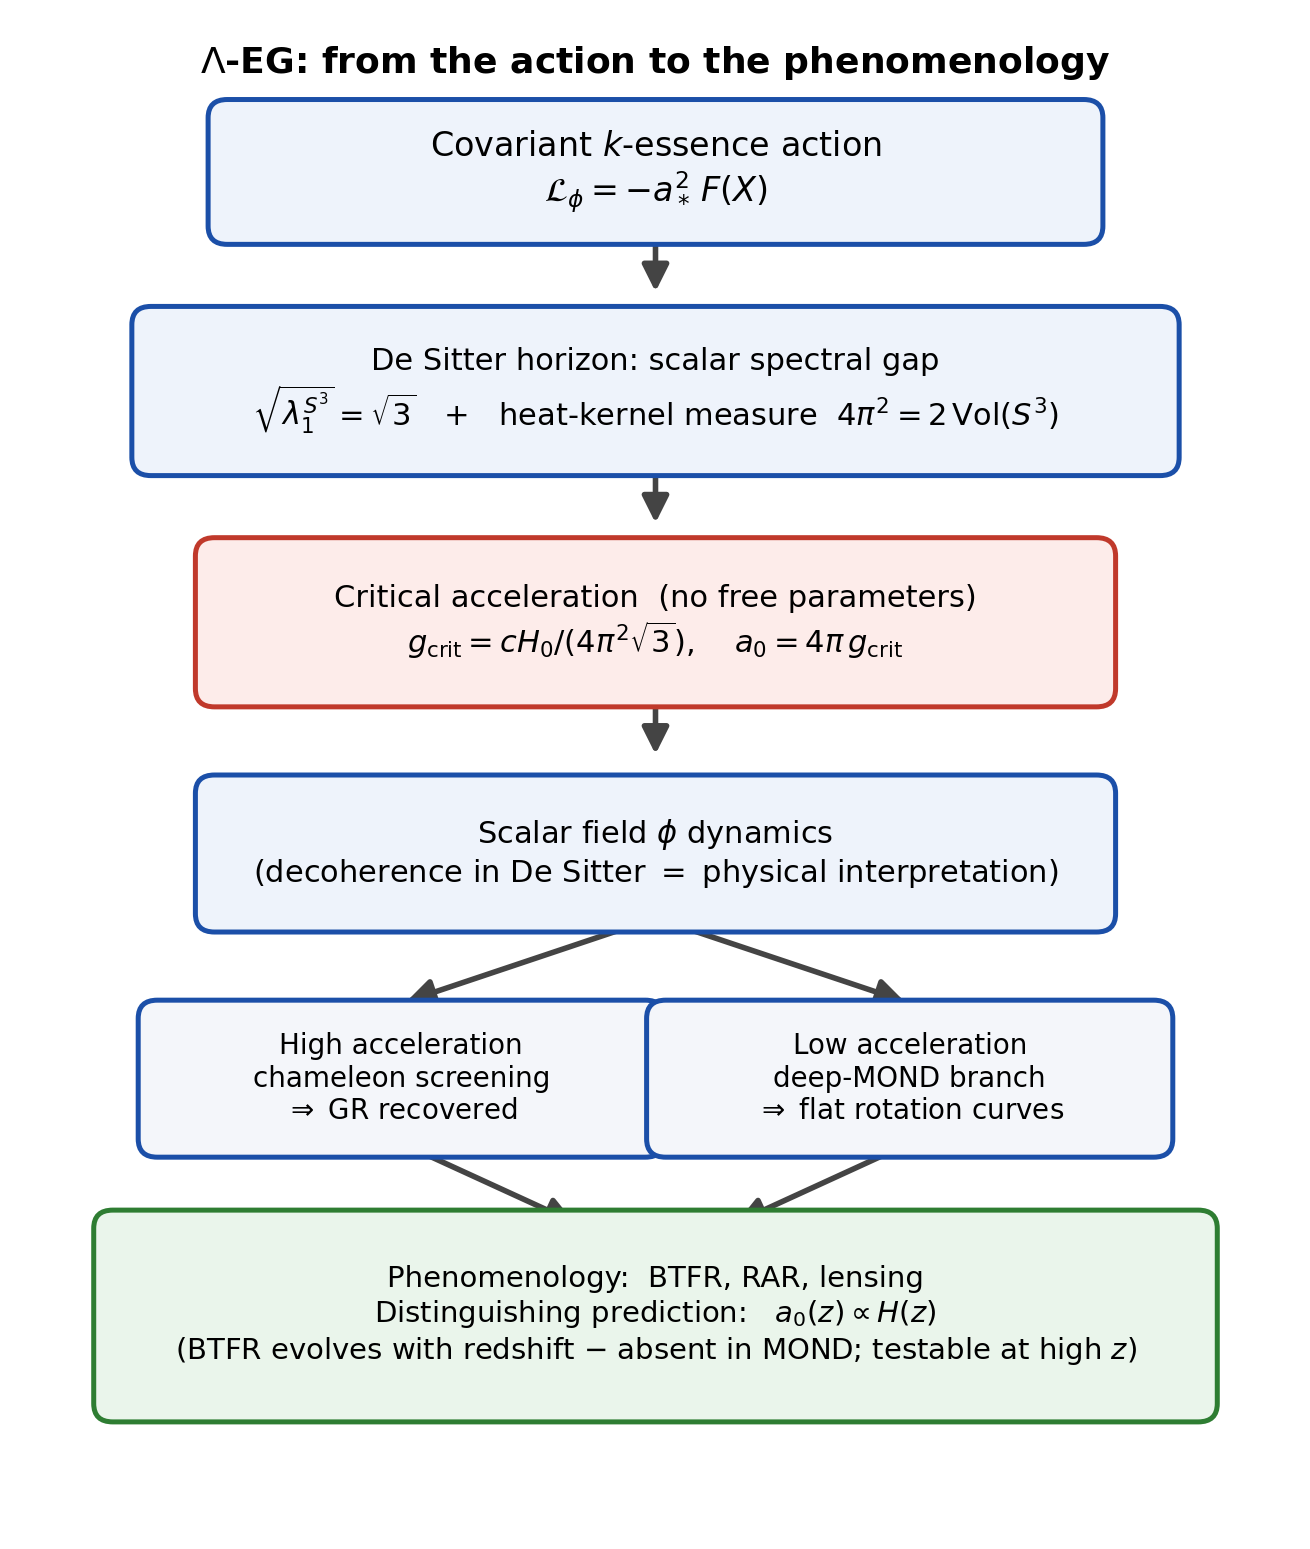
\includegraphics[width=0.78\textwidth]{fig6_concept.png}
\caption{%
  Logical structure of $\Lambda$-EG. The covariant $k$-essence action, evaluated on the
  De~Sitter horizon, fixes the critical acceleration $g_{\rm crit}$ from the scalar spectral
  gap and the heat-kernel measure (no free parameters). The scalar field then yields two
  regimes---chameleon screening (GR) at high acceleration and the deep-MOND branch at low
  acceleration---feeding the observational phenomenology. The distinguishing prediction is
  the redshift evolution $a_0(z)\propto H(z)$, absent in MOND.}
\label{fig:concept}
\end{figure}

\begin{figure}[ht]
\centering
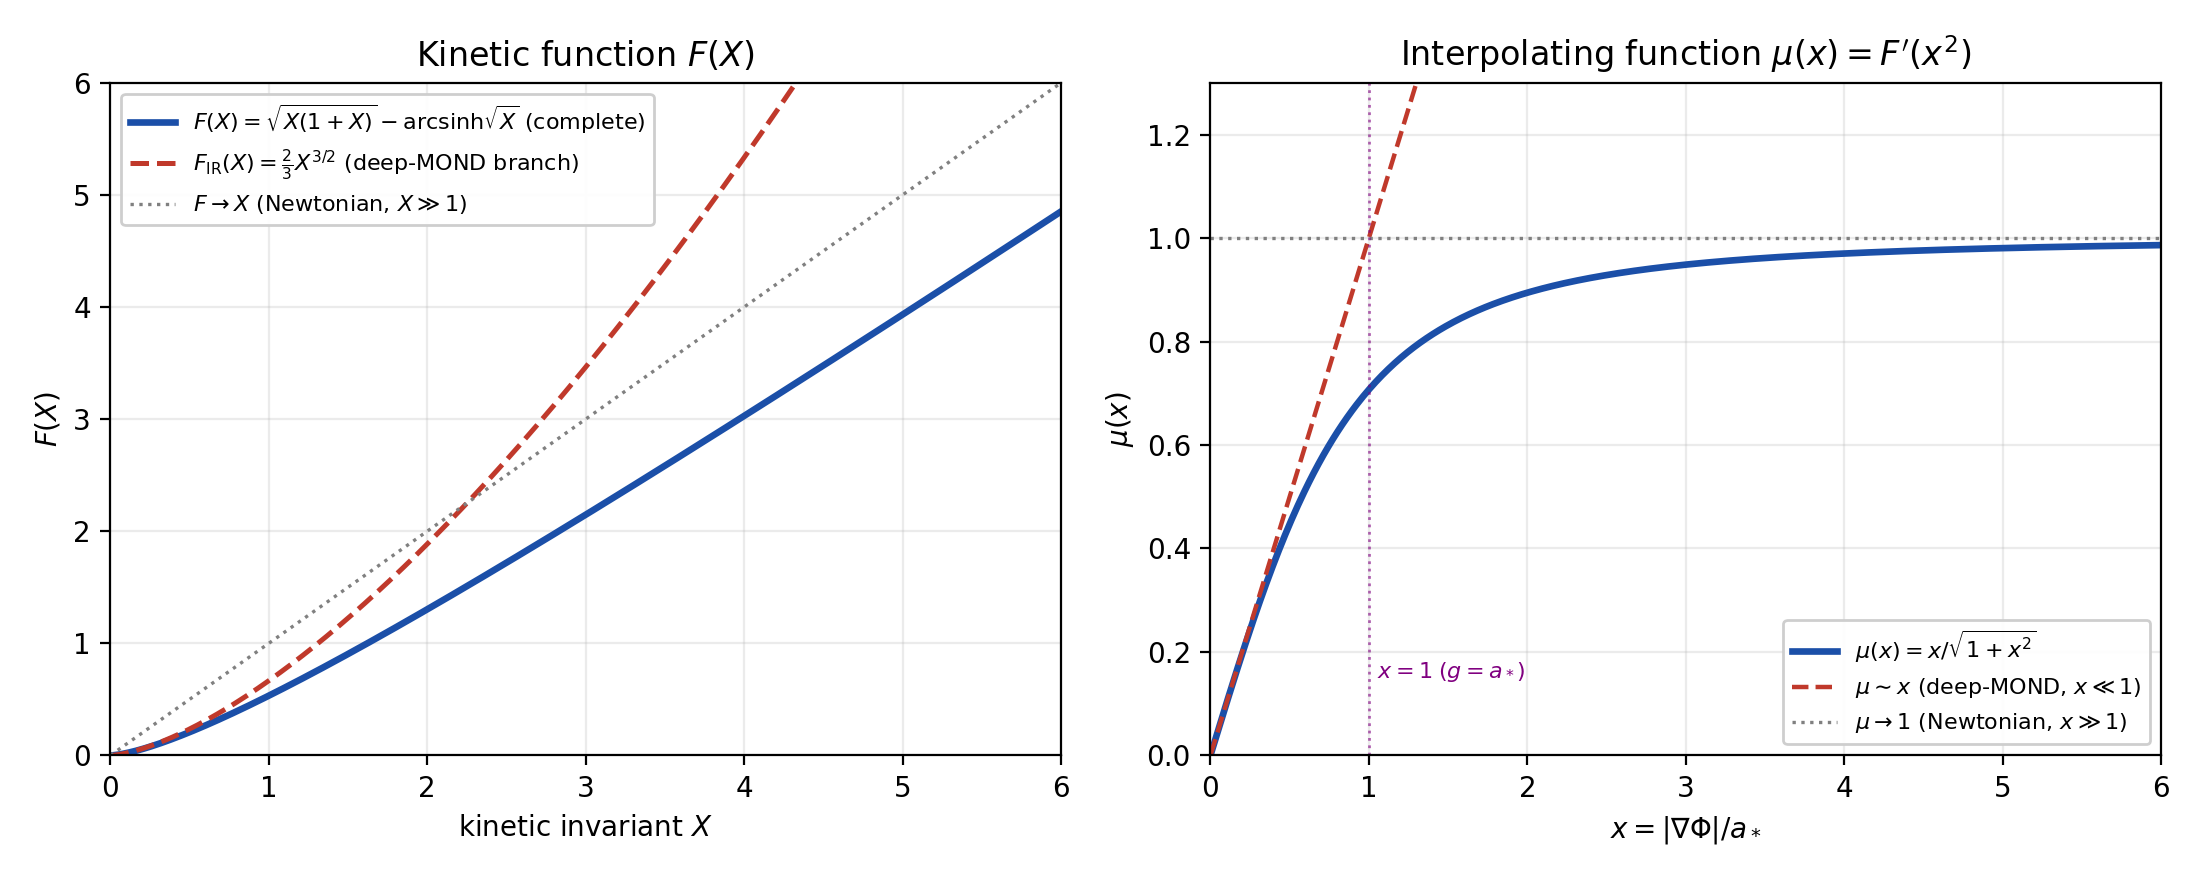
\includegraphics[width=0.95\textwidth]{fig5_F_mu.png}
\caption{%
  Kinetic function $F(X)$ (left) and interpolating function $\mu(x)=F'(x^2)$ (right).
  The pure branch $F_{\rm IR}=\tfrac{2}{3}X^{3/2}$ (dashed) captures only the deep-MOND
  limit, giving $\mu\sim x$; the complete kinetic function
  $F(X)=\sqrt{X(1+X)}-\mathrm{arcsinh}\sqrt{X}$ (solid) interpolates to Newtonian dynamics
  ($F\to X$, $\mu\to1$) at high acceleration, giving $\mu(x)=x/\sqrt{1+x^2}$. The critical
  point $x=1$ corresponds to $g=a_*$.}
\label{fig:Fphi}
\end{figure}

\begin{figure}[ht]
\centering
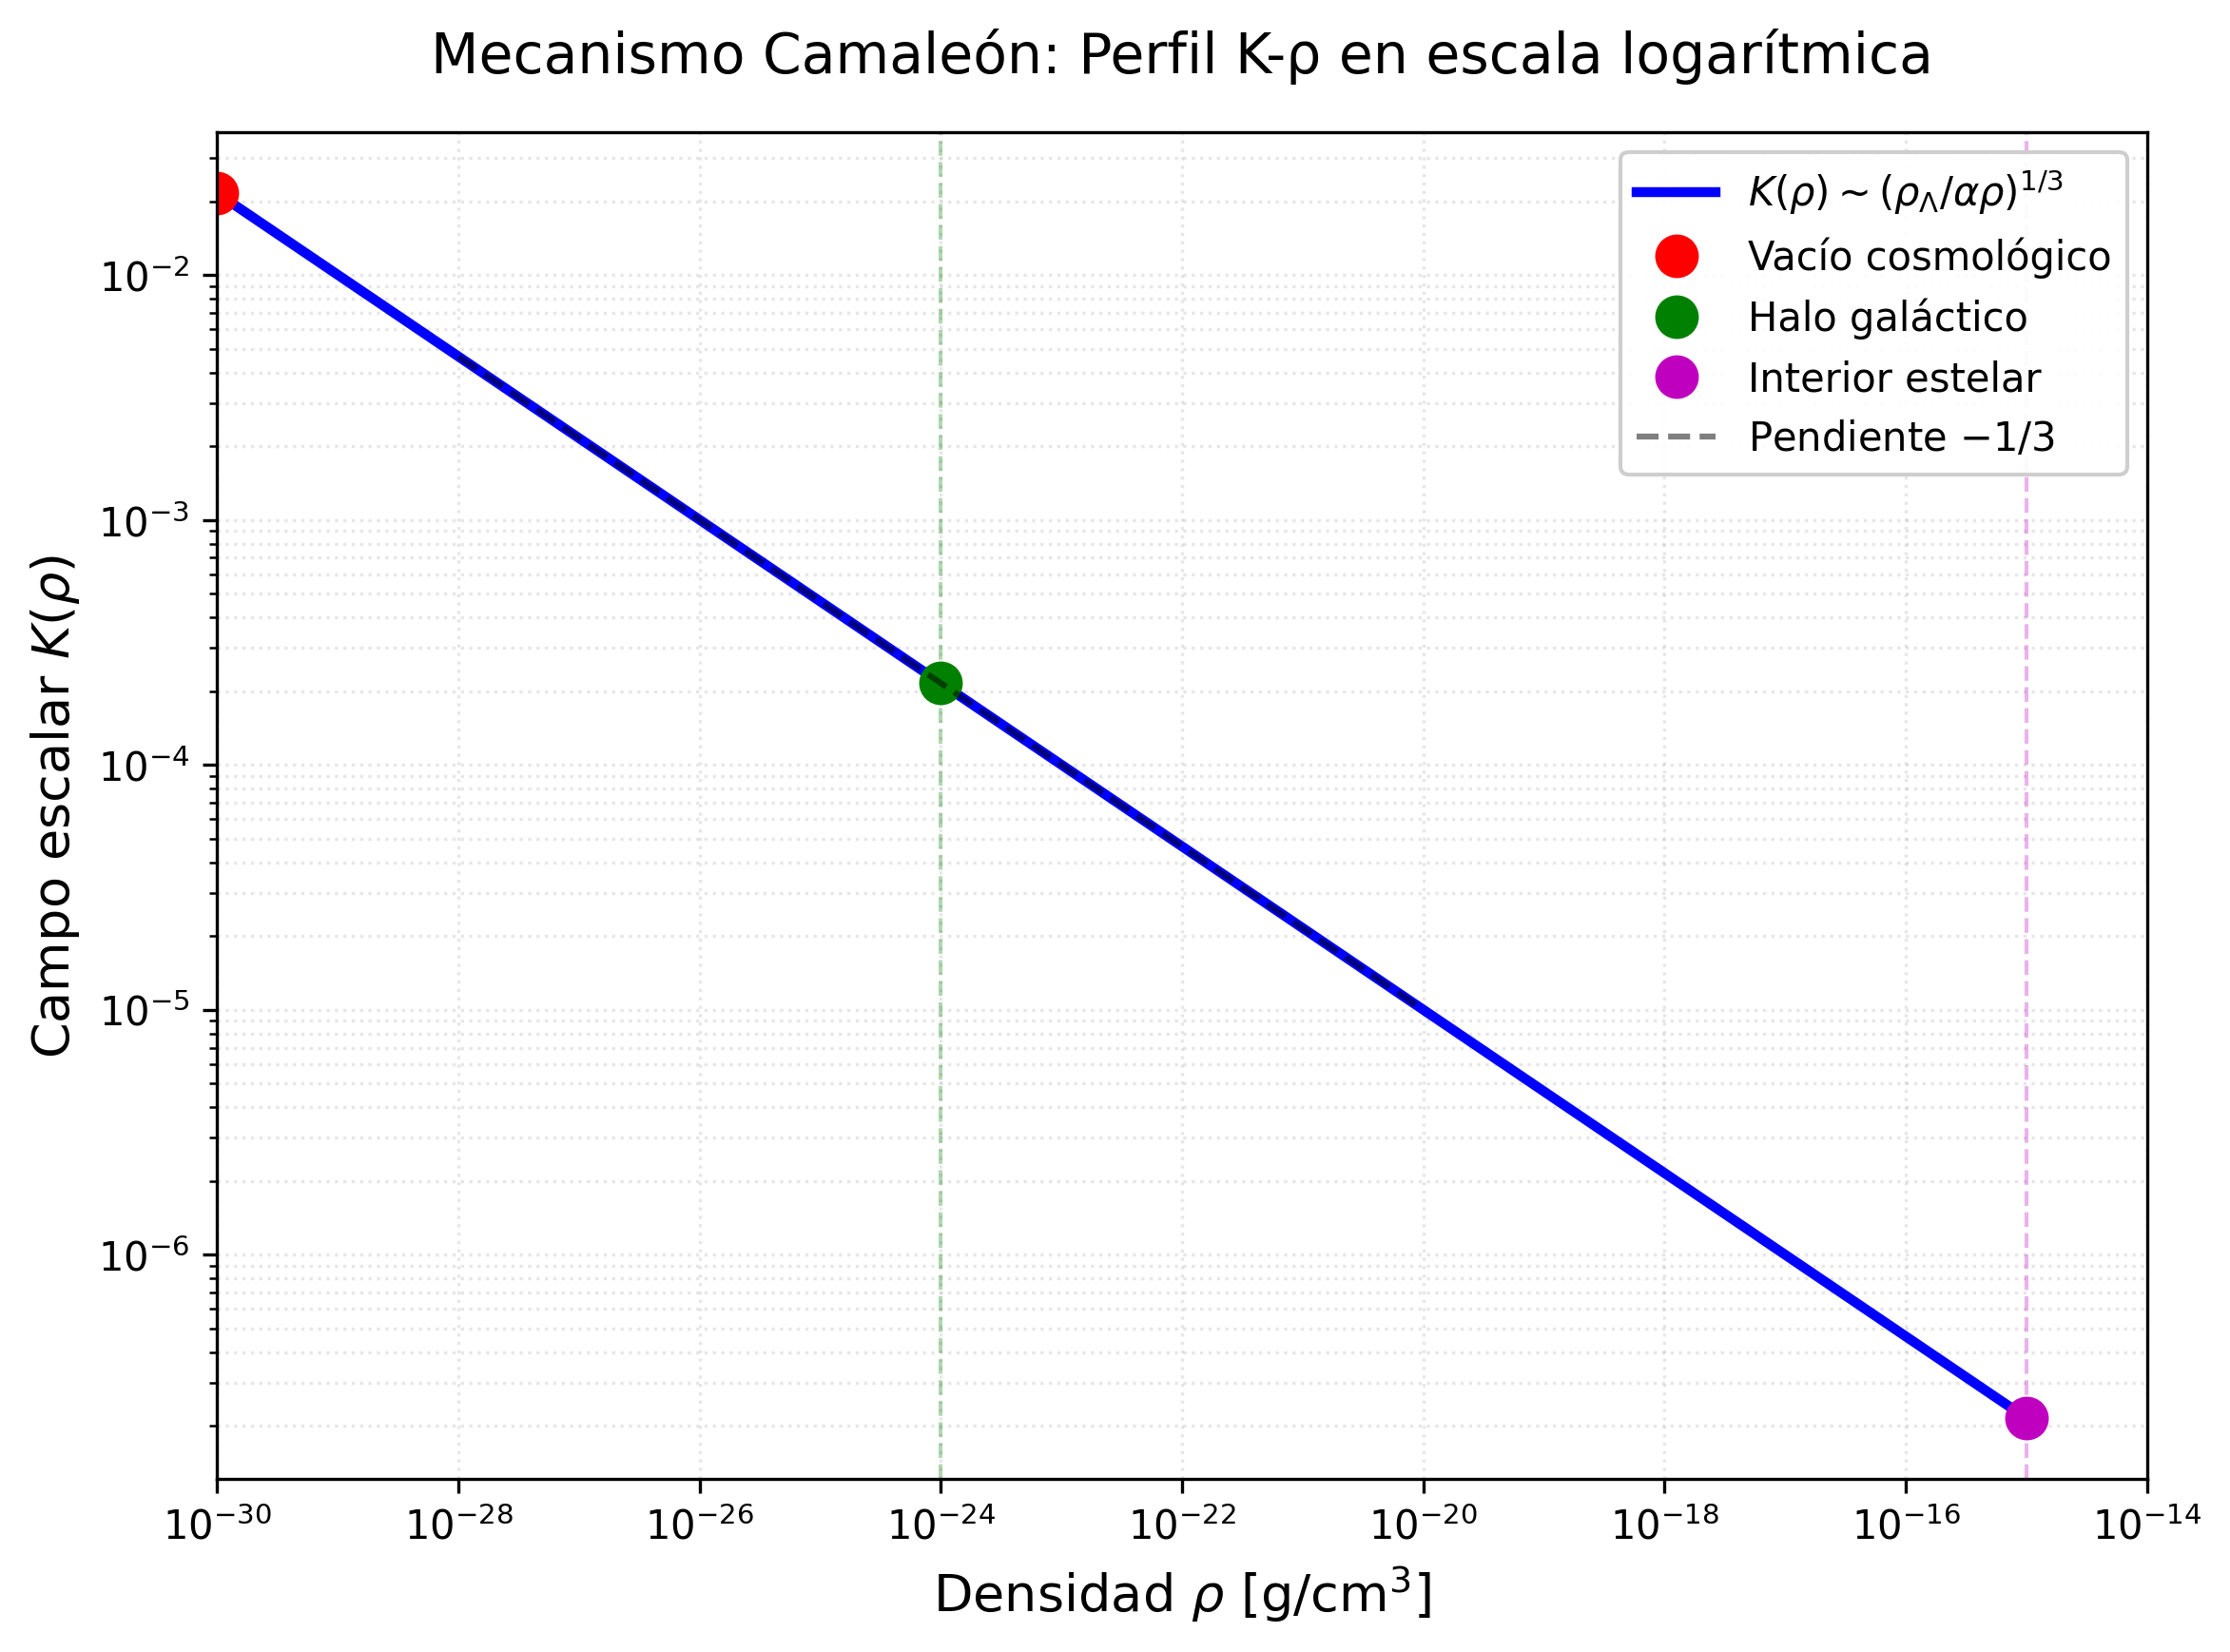
\includegraphics[width=0.85\textwidth]{fig1_K_rho_loglog.png}
\caption{%
  Chameleon profile $\phi_{\rm min}(\rho)\sim(\rho_\Lambda/\alpha\rho)^{1/3}$ in
  log-log scale. The slope $-1/3$ confirms the power-law scaling across 15 decades
  in density. Three characteristic environments are marked: cosmological void
  ($\rho\sim10^{-30}$~g\,cm$^{-3}$), galactic halo ($\rho\sim10^{-24}$~g\,cm$^{-3}$),
  and stellar interior ($\rho\sim10^{-15}$~g\,cm$^{-3}$). The strong suppression
  at high density is the mechanism underlying Solar-System viability.}
\label{fig:Krho}
\end{figure}

\begin{figure}[ht]
\centering
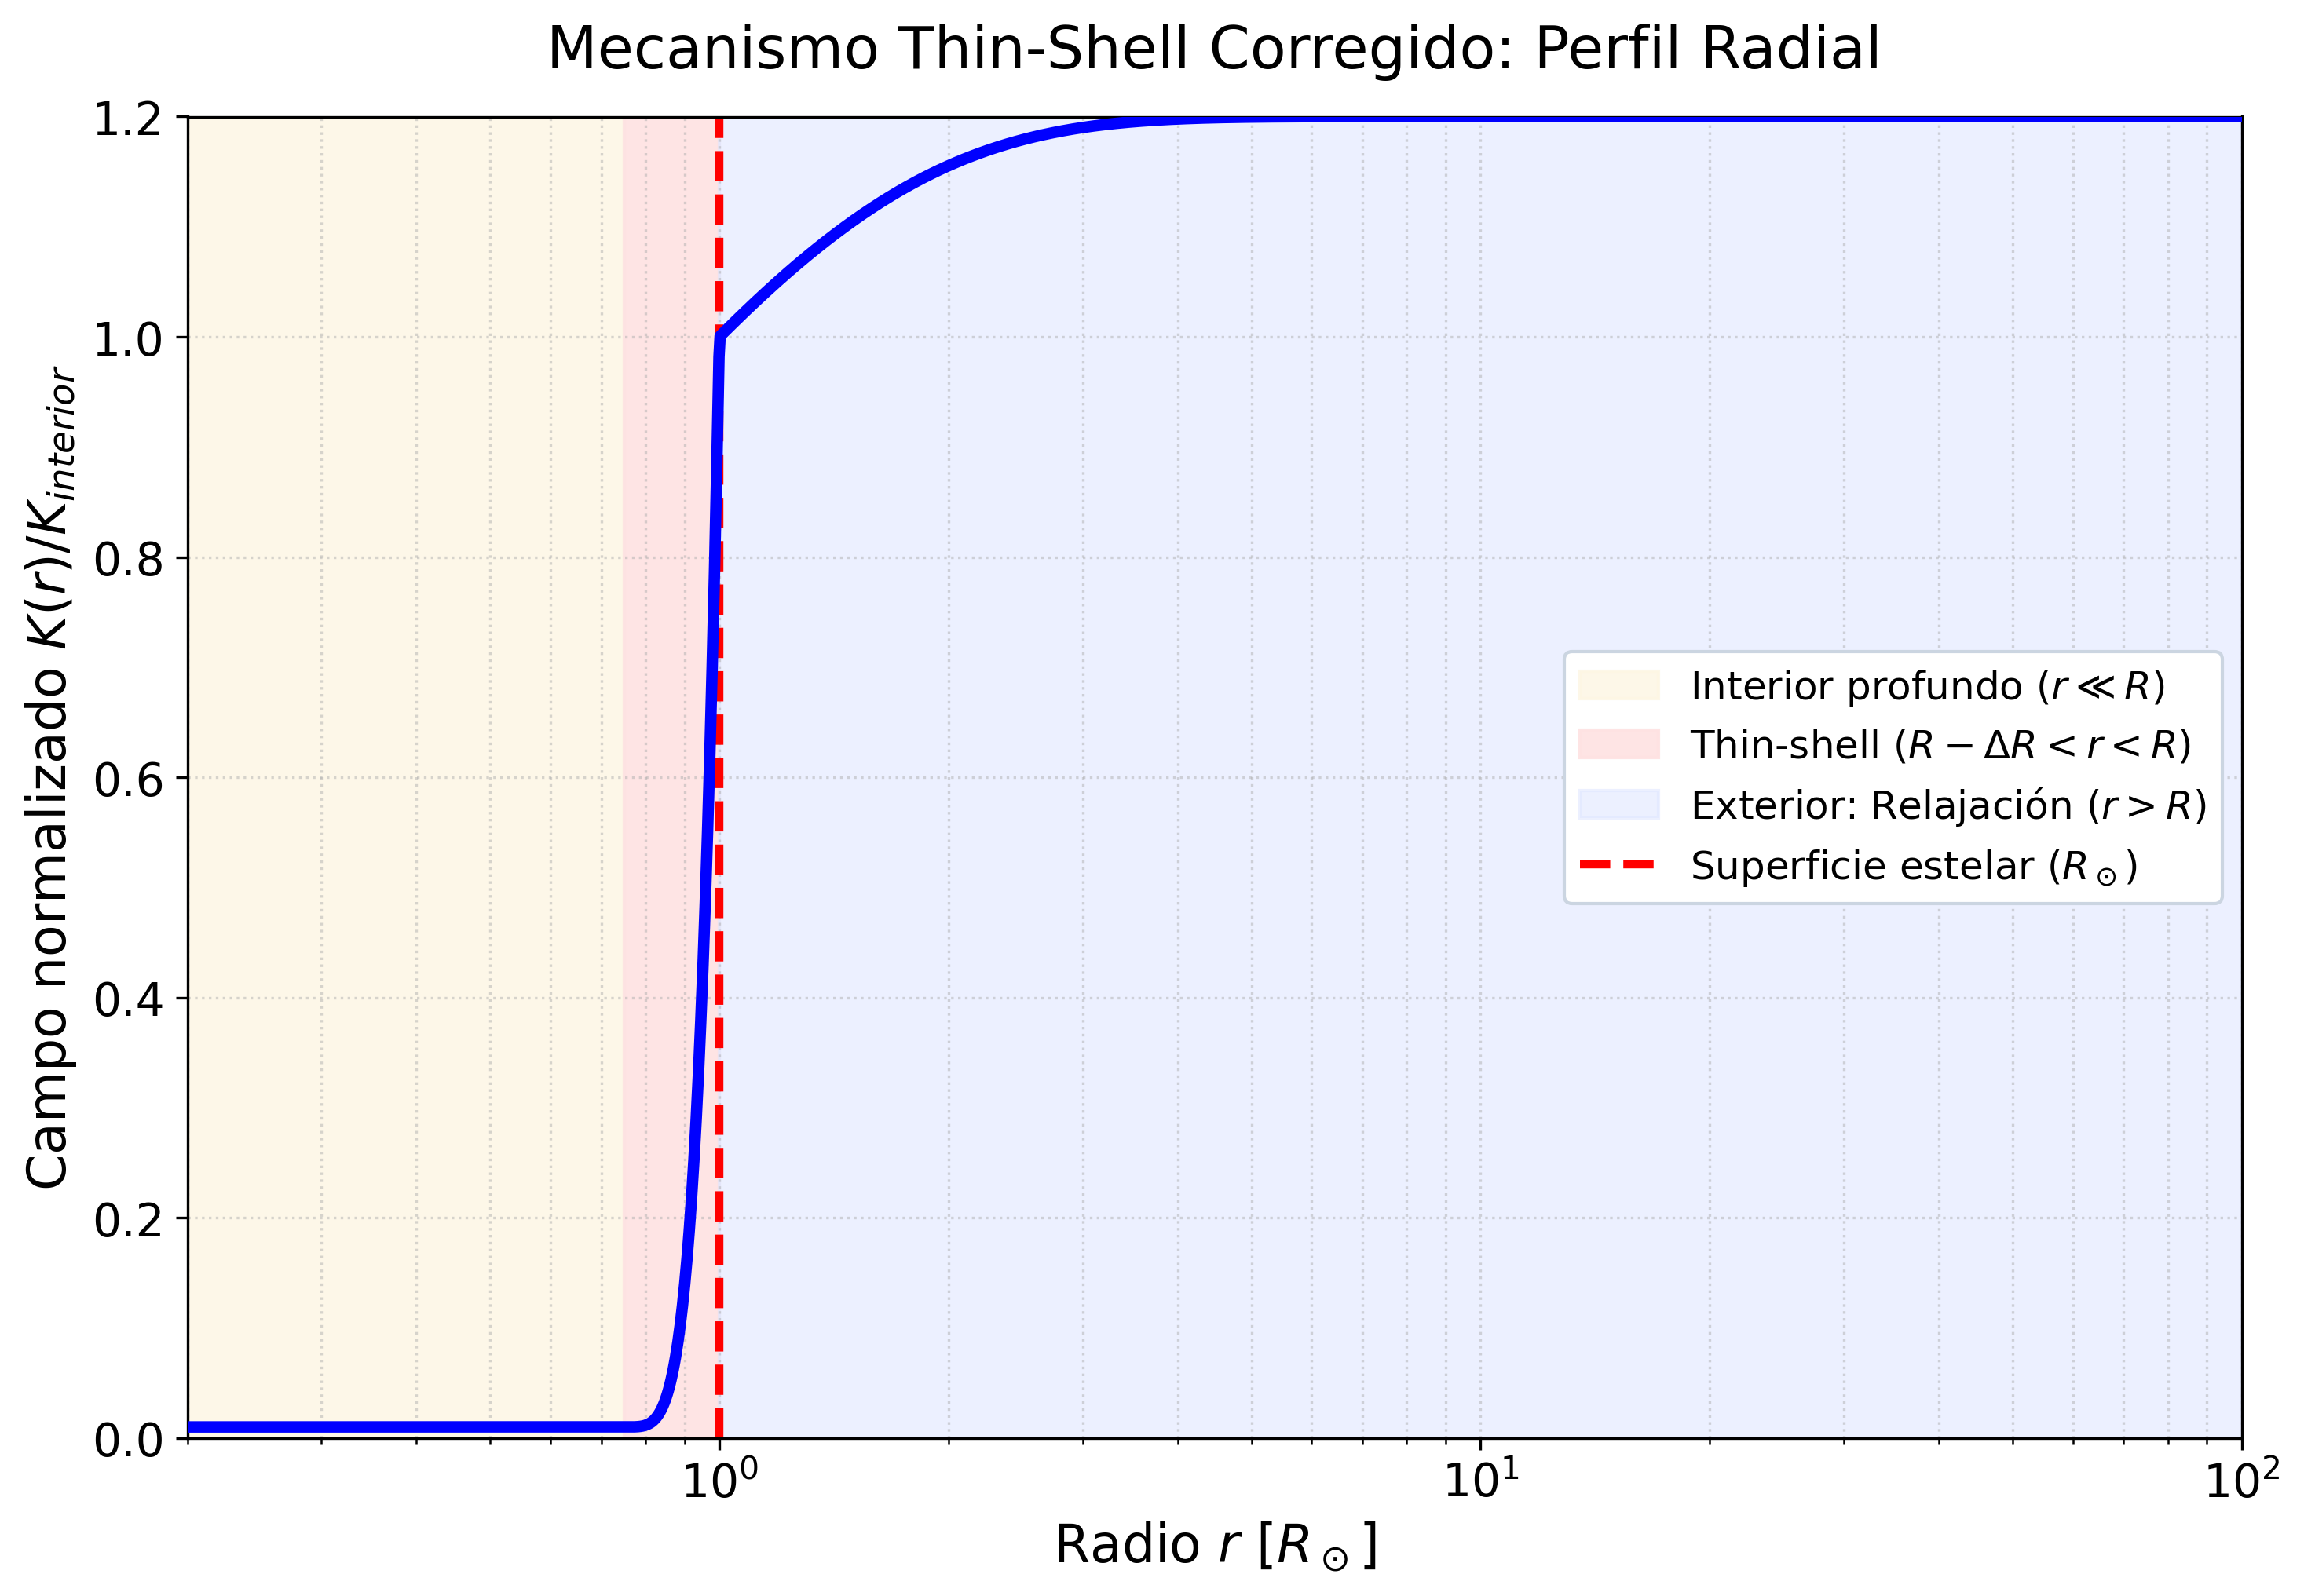
\includegraphics[width=0.85\textwidth]{fig2_K_r_thinshell_corregida.png}
\caption{%
  Radial profile of the normalized scalar field $\phi(r)/\phi_{\rm int}$ for a
  solar-type object. The strongly screened interior ($r\ll R_\odot$), the thin-shell
  transition region ($R_\odot-\Delta R < r < R_\odot$), and the exterior relaxation
  ($r > R_\odot$) are indicated. Only the thin-shell layer contributes to the exterior
  scalar force, enabling PPN compatibility.}
\label{fig:thinshell}
\end{figure}

\begin{figure}[ht]
\centering
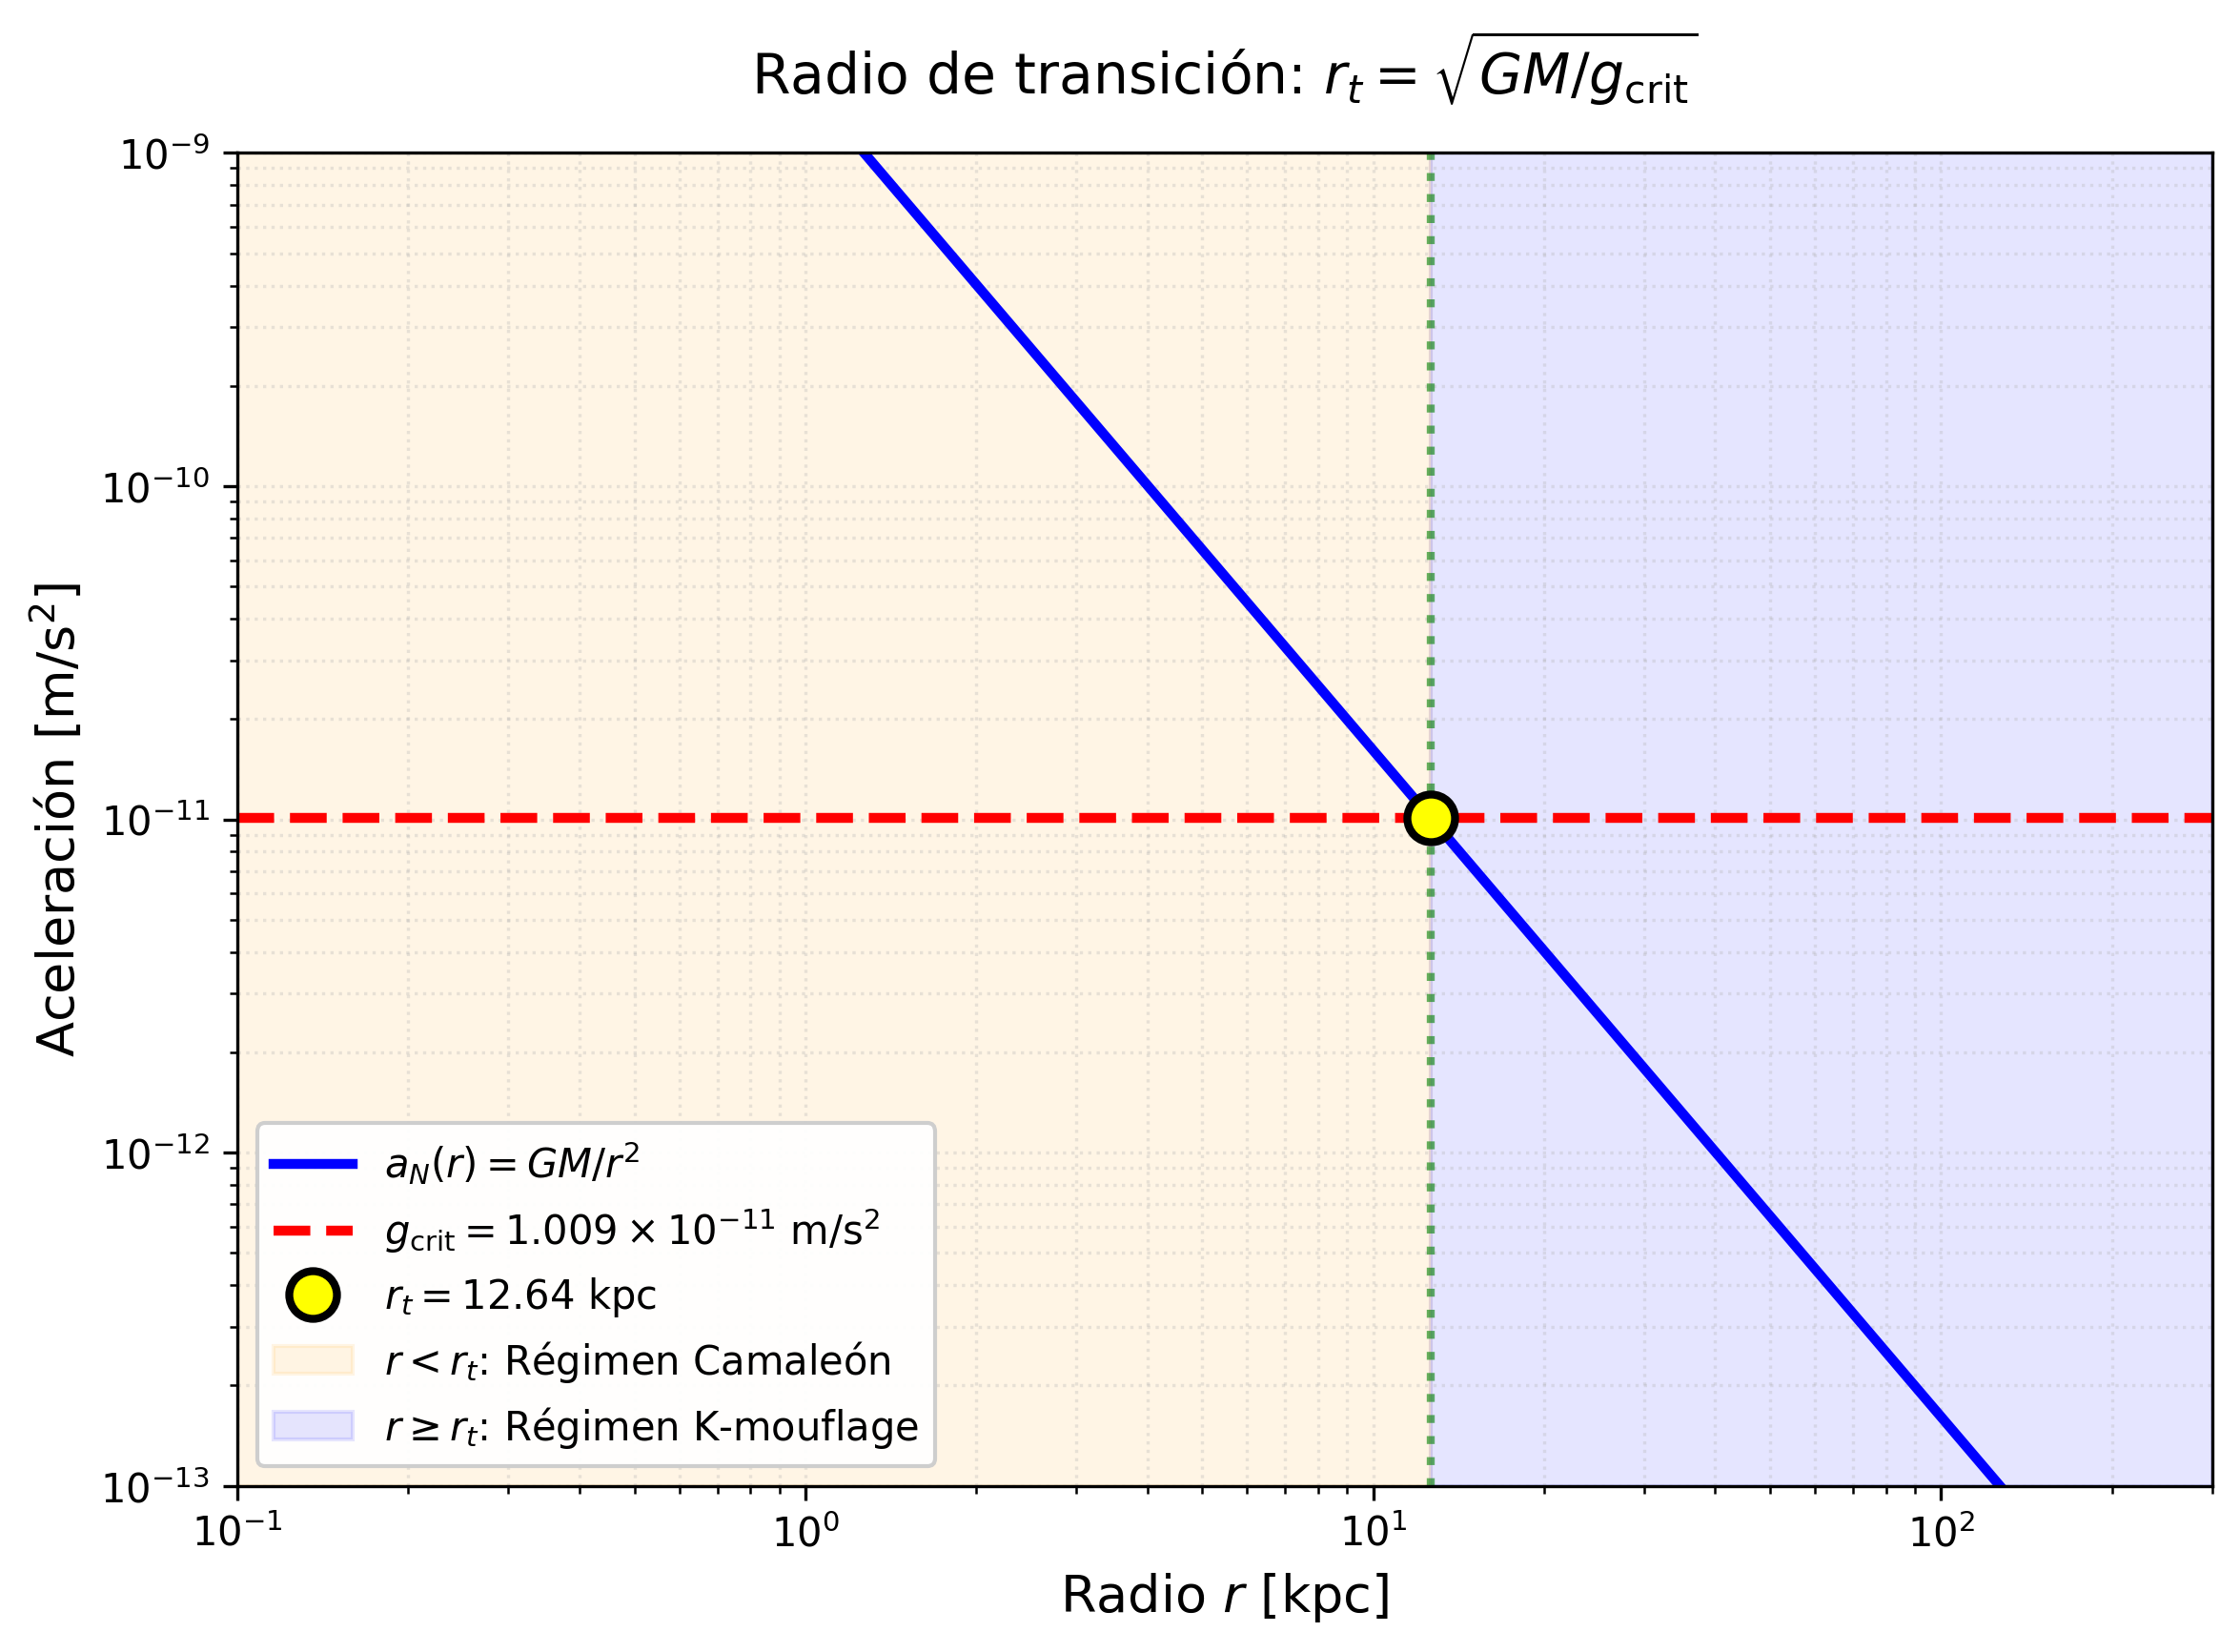
\includegraphics[width=0.85\textwidth]{fig3_r_transition.png}
\caption{%
  Determination of the topological transition radius $r_t = \sqrt{GM/g_{\rm crit}}$.
  The Newtonian acceleration $a_N(r) = GM/r^2$ (solid curve) intersects the
  critical scale $g_{\rm crit} = 9.58\times10^{-12}$~m\,s$^{-2}$ (dashed line) at
  $r_t\approx12.6$~kpc for $M = 2.3\times10^{10}\,M_\odot$.
  For $r < r_t$ (shaded, Chameleon regime), screening dominates; for $r\geq r_t$
  (blue, k-mouflage/AQUAL regime), the kinetic branch governs.}
\label{fig:rt}
\end{figure}

\begin{figure}[ht]
\centering
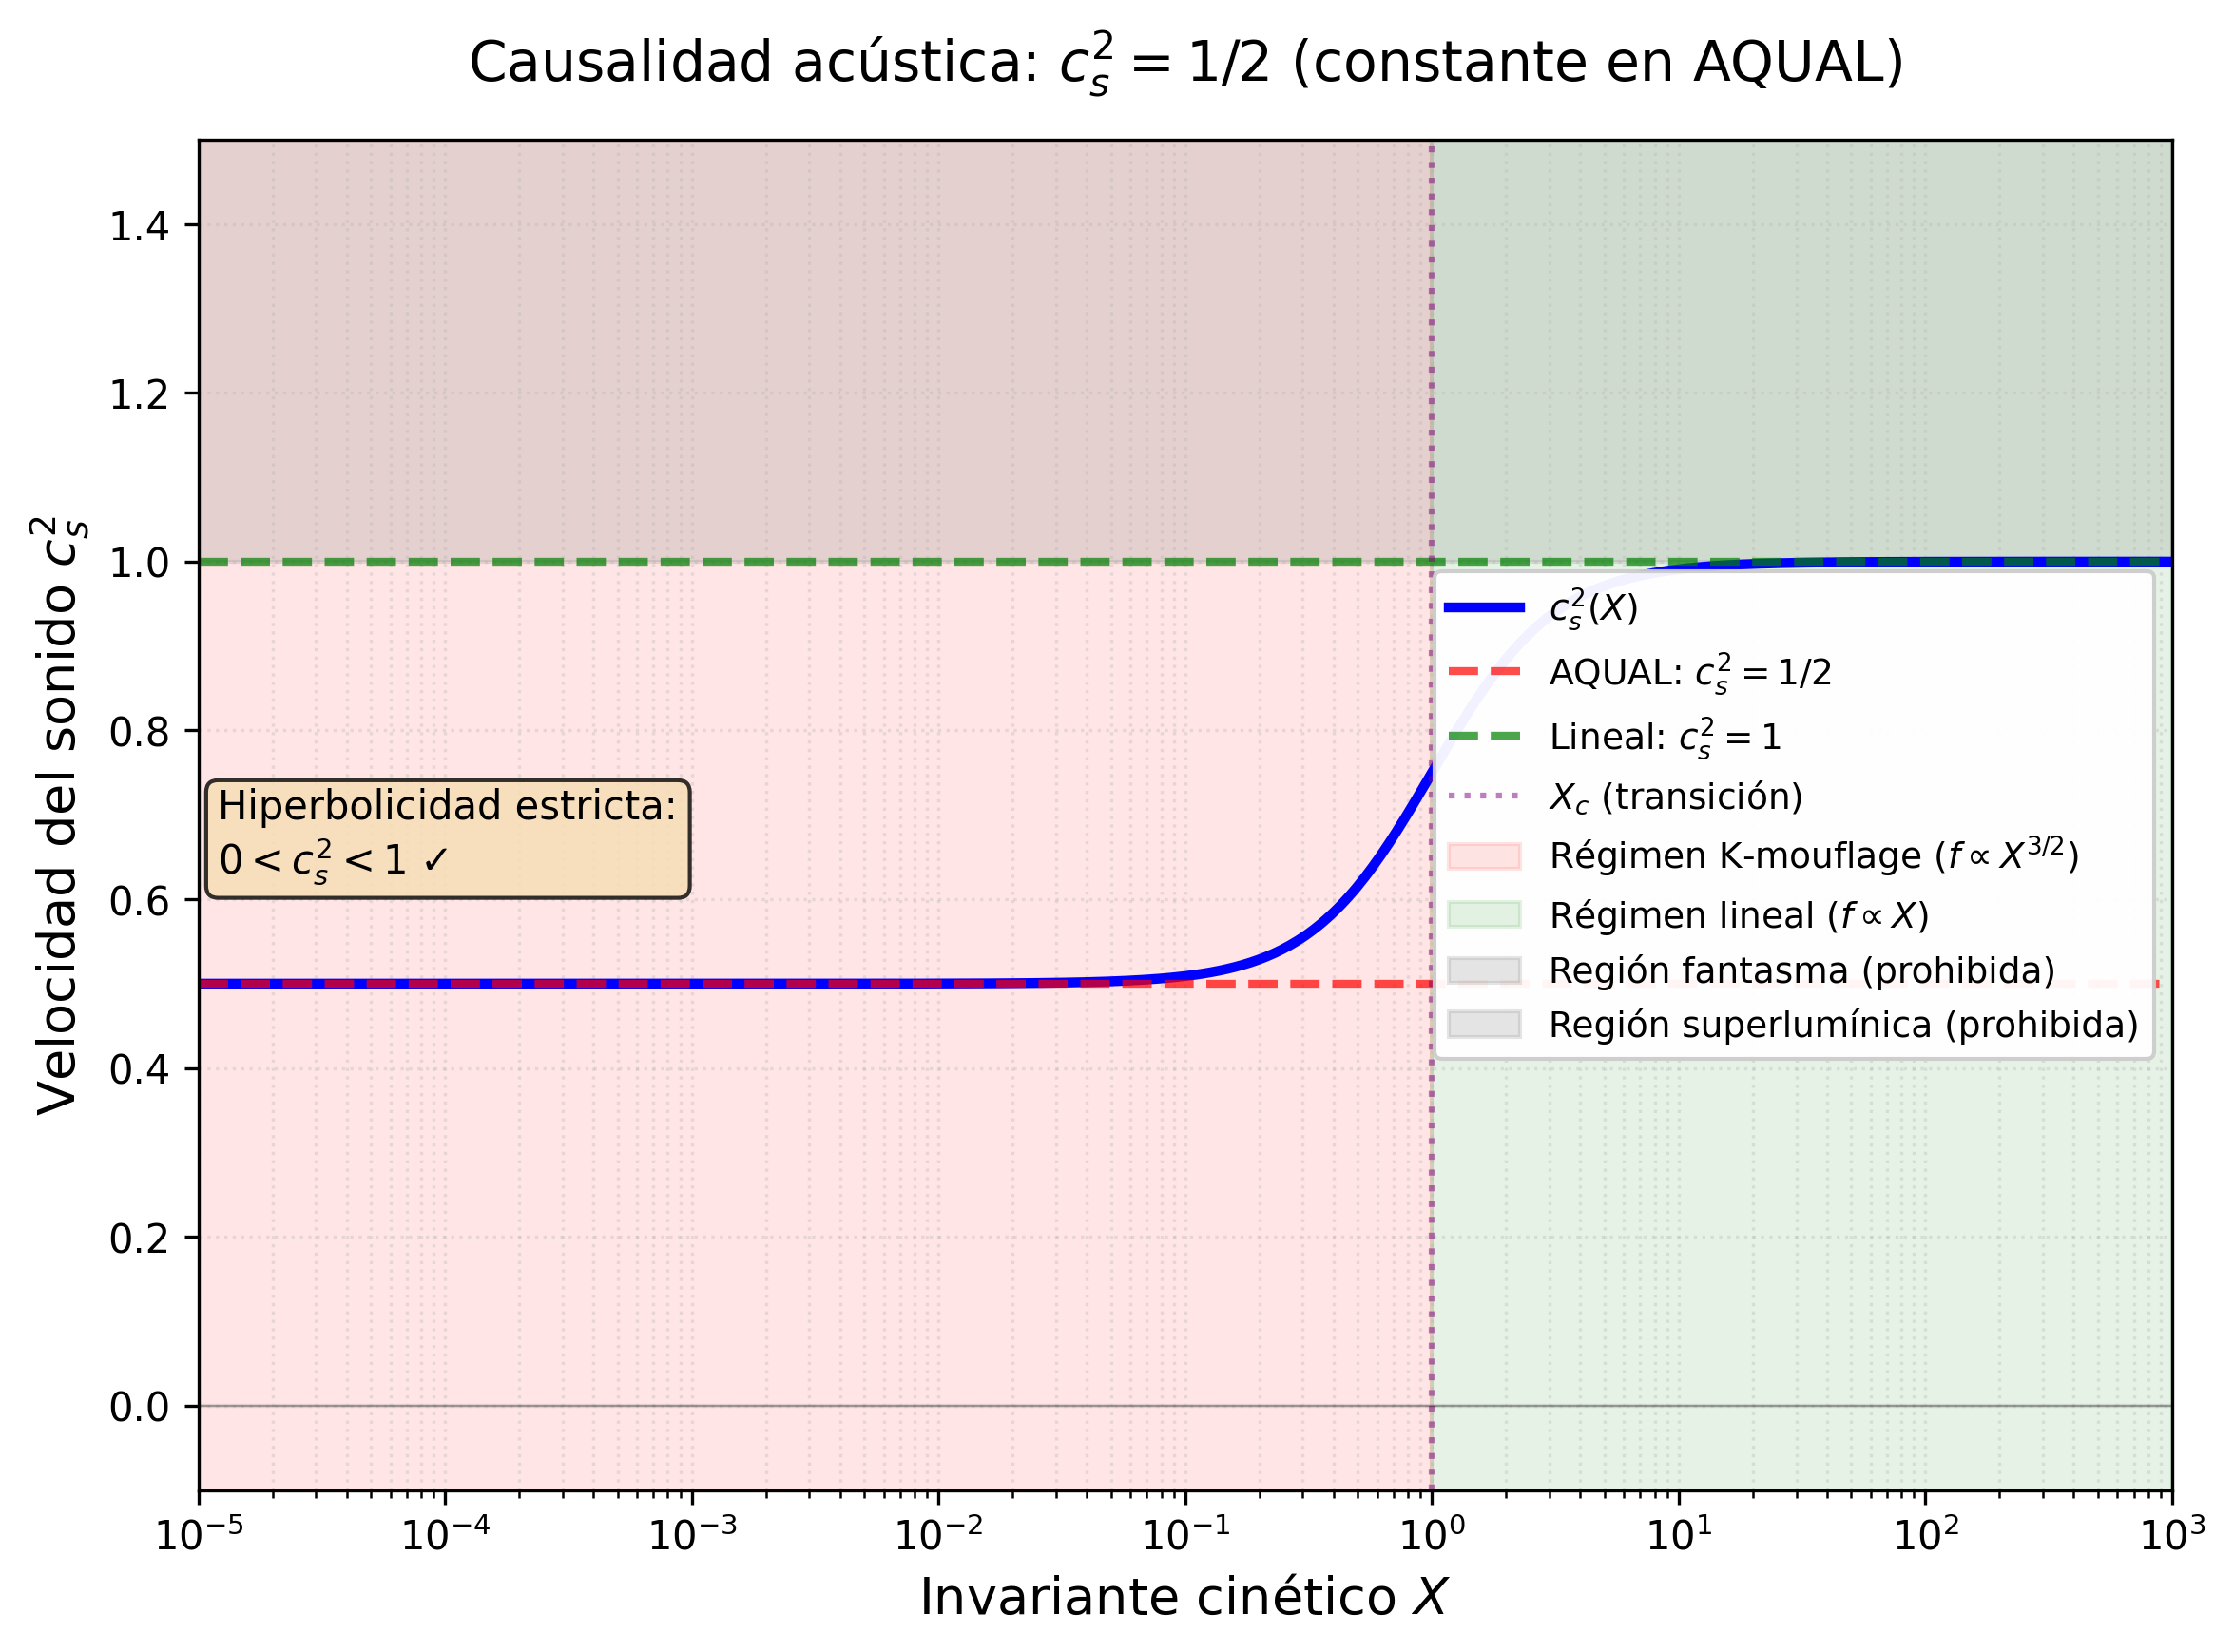
\includegraphics[width=0.85\textwidth]{fig4_cs2_vs_X.png}
\caption{%
  Effective sound speed $c_s^2$ as a function of the kinetic invariant $X$.
  In the AQUAL/k-mouflage regime ($X\ll X_c$, relevant to galactic scales),
  $c_s^2 = 1/2$ exactly. In the Newtonian limit ($X\gg X_c$, Solar-System scales),
  $c_s^2\to 1$. The permitted causal region $0 < c_s^2 < 1$ ensures strict
  hyperbolicity and the absence of ghost instabilities throughout.}
\label{fig:cs2}
\end{figure}

%%====================================================
\begin{thebibliography}{99}

\bibitem{Clowe2006}
  D.~Clowe et al.,
  Astrophys.\ J.\ Lett.\ \textbf{648}, L109 (2006).

\bibitem{PaperI}
  J.~P.~Figueroa Torres,
  ``Emergent Gravity from De~Sitter Coherence: Derivation of $g_{\rm crit}$,
  Dual-Regime Galactic Dynamics, and Cosmological Evolution of the BTFR,''
  Paper~I (2026), in preparation.

\bibitem{PaperII}
  J.~P.~Figueroa Torres,
  ``Off-Equilibrium Coherence Dynamics: Inertial Lag and the Bullet Cluster
  without Dark Matter,''
  Paper~II (2026), in preparation.

\bibitem{Milgrom1983}
  M.~Milgrom,
  Astrophys.\ J.\ \textbf{270}, 365 (1983).

\bibitem{Bekenstein1984}
  J.~D.~Bekenstein and M.~Milgrom,
  Astrophys.\ J.\ \textbf{286}, 7 (1984).

\bibitem{Bekenstein2004}
  J.~D.~Bekenstein,
  Phys.\ Rev.\ D \textbf{70}, 083509 (2004).

\bibitem{Khoury2004}
  J.~Khoury and A.~Weltman,
  Phys.\ Rev.\ Lett.\ \textbf{93}, 171104 (2004).

\bibitem{Babichev2009}
  E.~Babichev, C.~Deffayet, and R.~Ziour,
  Int.\ J.\ Mod.\ Phys.\ D \textbf{18}, 2147 (2009).

\bibitem{Verlinde2017}
  E.~Verlinde,
  SciPost Phys.\ \textbf{2}, 016 (2017).

\bibitem{McGaugh2000}
  S.~S.~McGaugh, J.~M.~Schombert, G.~D.~Bothun, and W.~J.~G.~de~Blok,
  Astrophys.\ J.\ Lett.\ \textbf{533}, L99 (2000).

\bibitem{McGaugh2016}
  S.~S.~McGaugh, F.~Lelli, and J.~M.~Schombert,
  Phys.\ Rev.\ Lett.\ \textbf{117}, 201101 (2016).

\bibitem{Rubin1980}
  V.~C.~Rubin, W.~K.~Ford, and N.~Thonnard,
  Astrophys.\ J.\ \textbf{238}, 471 (1980).

\bibitem{ArmendarizPicon1999}
  C.~Armend\'ariz-Pic\'on, T.~Damour, and V.~Mukhanov,
  Phys.\ Lett.\ B \textbf{458}, 209 (1999).

\bibitem{Gibbons1977}
  G.~W.~Gibbons and S.~W.~Hawking,
  Phys.\ Rev.\ D \textbf{15}, 2738 (1977).

\bibitem{Bunch1978}
  T.~S.~Bunch and P.~C.~W.~Davies,
  Proc.\ R.\ Soc.\ Lond.\ A \textbf{360}, 117 (1978).

\bibitem{Bertotti2003}
  B.~Bertotti, L.~Iess, and P.~Tortora,
  Nature \textbf{425}, 374 (2003).

\bibitem{Will2014}
  C.~M.~Will,
  Living Rev.\ Rel.\ \textbf{17}, 4 (2014).

\bibitem{Woodard2007}
  R.~P.~Woodard,
  Lect.\ Notes Phys.\ \textbf{720}, 403 (2007).

\bibitem{Lelli2016}
  F.~Lelli, S.~S.~McGaugh, and J.~M.~Schombert,
  Astron.\ J.\ \textbf{152}, 157 (2016).

\bibitem{Hunter2012}
  D.~A.~Hunter et al.,
  Astron.\ J.\ \textbf{144}, 134 (2012).

\bibitem{Planck2020}
  Planck Collaboration,
  Astron.\ Astrophys.\ \textbf{641}, A6 (2020).

\bibitem{Clifton2012}
  T.~Clifton, P.~G.~Ferreira, A.~Padilla, and C.~Skordis,
  Phys.\ Rep.\ \textbf{513}, 1 (2012).

\end{thebibliography}

\end{document}
